%%
%% FGCS submission — Elsevier CAS bundle (double column)
%% Converted from elsarticle to cas-dc. Content preserved; LaTeX/template-only changes.
%%
\documentclass[a4paper,fleqn]{cas-dc}

\usepackage[numbers]{natbib}
\usepackage{amsmath}
\usepackage{amssymb}
\usepackage{placeins}
\usepackage{float}
\usepackage{capt-of}

\begin{document}
\let\WriteBookmarks\relax
\def\floatpagepagefraction{1}
\def\textpagefraction{.001}

\shorttitle{Hybrid ML for Multi-Metric Prediction in the Cloud--Edge Continuum}
\shortauthors{A. Kadouma et al.}

\title[mode=title]{Hybrid Machine Learning for Real-Time Multi-Metric Application Behavior Prediction in the Cloud--Edge Continuum}

\author[1]{Abdelhak Kadouma}
\cormark[1]
\ead{abdelhak.kadouma@uwasa.fi}
\credit{Conceptualization, Methodology, Software, Data curation, Formal analysis, Validation, Visualization, Writing -- original draft}

\author[1]{Amit Shukla}
\ead{amit.shukla@uwasa.fi}
\credit{Supervision, Conceptualization, Methodology, Writing -- review \& editing}

\author[1]{Mohammed Elmusrati}
\ead{moel@uwasa.fi}
\credit{Supervision, Project administration, Funding acquisition, Writing -- review \& editing}

\affiliation[1]{organization={University of Vaasa},
            city={Vaasa},
            country={Finland}}

\cortext[1]{Corresponding author}

\begin{abstract}
Applications deployed across the Cloud--Edge Computing Continuum (CECC) exhibit highly dynamic and multi-dimensional resource usage patterns, and reactive monitoring and autoscaling mechanisms struggle to prevent SLA violations and inefficient resource utilization under rapidly changing workloads. This study aims to develop a real-time, per-VM prediction framework capable of accurately forecasting short-term resource behavior across multiple operational metrics in CECC environments. Using the large-scale GWA-T-13 Materna dataset comprising production-grade traces from over 1,500 virtual machines, we model four key metrics: CPU usage, memory usage, disk write throughput, and network throughput. A hybrid tree-based approach is introduced, combining Random Forest for smoother CPU and memory dynamics with XGBoost for burst-prone disk and network behavior, and an extensive feature-engineering pipeline incorporating lag features, rolling statistics, and temporal encodings supports the modeling process. The proposed framework achieves strong predictive accuracy, with $R^2$ values of approximately 0.95 for CPU, 0.89 for memory, 0.94 for disk throughput, and 0.91 for network throughput, demonstrating that aligning model families with metric-specific statistical properties significantly improves short-horizon forecasting performance. The hybrid prediction framework provides an effective foundation for proactive CECC orchestration; by integrating forecasts into dynamic Application Profile Models (APMs), the approach enables anticipatory autoscaling, latency-aware placement, and SLA-sensitive lifecycle management, advancing predictive intelligence in distributed cloud--edge systems.
\end{abstract}

\begin{highlights}
\item Hybrid RF--XGBoost models predict CECC resource behavior.
\item The framework forecasts CPU, memory, disk, and network metrics.
\item GWA-T-13 Materna traces validate VM-level prediction accuracy.
\item Metric-aware model choice improves short-horizon forecasting.
\item Forecasts support proactive cloud--edge orchestration.
\end{highlights}

\begin{keywords}
Cloud--Edge Computing Continuum \sep Application Performance Prediction \sep Machine Learning \sep Time-Series Forecasting \sep Hybrid Tree-Based Models \sep Random Forest \sep XGBoost \sep Resource Usage Prediction \sep Proactive Orchestration
\end{keywords}

\maketitle

\section{Introduction}
\label{sec:introduction}

The rapid evolution of distributed systems has led to the emergence of the Cloud--Edge Computing Continuum (CECC), a paradigm in which computation, storage, and networking resources are seamlessly integrated across centralized clouds, regional edge platforms, and far-edge devices located close to users, machines, or sensors. This continuum enables latency-sensitive and resource-intensive applications---including real-time video analytics, industrial automation, autonomous systems, extended reality (XR), and intelligent transportation---to meet strict performance, responsiveness, and scalability requirements \cite{b1,b2}. To support these demands, modern applications increasingly adopt microservices-based designs, decomposing functionality into independently deployable components that can be dynamically placed across heterogeneous infrastructure layers according to workload characteristics, SLAs, and operational constraints \cite{b3}.

However, the transition from centralized cloud computing to CECC significantly increases operational complexity. Microservices deployed across heterogeneous environments generate highly dynamic, multi-metric workload patterns: CPU utilization fluctuates with computation bursts, memory usage varies with data dependencies, network throughput changes due to traffic conditions, and application throughput responds to user demand cycles. These metrics interact in non-linear ways, influenced by virtualization overhead, container orchestration, resource contention, and temporal access patterns \cite{b4}. Unlike traditional cloud environments, CECC workloads often exhibit heavy-tailed distributions, strong burstiness, and extreme skewness---particularly in disk and network metrics---making them difficult to predict using simplistic or reactive monitoring tools \cite{b5}. Furthermore, many performance indicators in CECC show weak long-term temporal dependencies, meaning that long-sequence neural architectures may not yield consistent benefits over well-engineered statistical or ensemble models \cite{b6}.

Despite advances in cloud monitoring systems, current CECC orchestration remains predominantly reactive. Standard autoscaling tools detect threshold violations and anomalies only after resource saturation occurs, causing SLA degradation, latency spikes, and user-perceived performance loss \cite{b7}. Existing research on resource prediction has explored machine learning models for CPU, memory, or network forecasting, but several limitations persist. First, prior work focuses mainly on predicting a single resource metric---typically CPU---while overlooking the multi-metric nature of CECC performance \cite{b8}. Second, many prediction approaches assume homogeneous cloud settings and do not generalize to the heterogeneous environments that characterize CECC. Third, most studies operate at coarse granularity (cluster or host level), whereas CECC orchestration decisions (e.g., placement, scaling, migration) must be taken at VM or microservice granularity. As a result, current solutions lack the fine-grained, real-time predictive capabilities required to support proactive, SLA-aware decision-making.

Short-horizon, per-VM multi-metric prediction is therefore essential for CECC lifecycle management. Anticipating CPU increases enables preemptive scaling; predicting upcoming memory pressure avoids container eviction; forecasting network throughput supports placing bandwidth-intensive microservices at the optimal tier of the continuum; and anticipating throughput fluctuations helps avoid SLA violations during peak loads. Accurate short-term forecasts are particularly important because many CECC workloads are governed by operational cycles (e.g., business-hour peaks), bursty interactions, or sudden external triggers that require rapid adaptation. Such prediction must be lightweight, fast, and robust to the diverse statistical patterns exhibited by CECC telemetry.

Achieving effective prediction requires real-world datasets that capture production-grade behavior. For this purpose, we leverage the GWA-T-13 Materna dataset, one of the largest publicly available traces of VM-level operational metrics collected from a commercial enterprise datacenter. The dataset contains three month-long traces consisting of 520, 527, and 547 VMs, respectively, running business-critical workloads across a VMware ESX cluster with 49 hosts and 6780 GB RAM. The traces include detailed measurements of CPU capacity and usage, memory provisioning and usage, disk I/O throughput, and network throughput, recorded at fine temporal granularity. Unlike synthetic datasets, GWA-T-13 captures real operational variability, workload heterogeneity, heavy tails, bursts, and multi-metric interactions, making it highly suitable for rigorous prediction studies \cite{b9}. This dataset also exposes the practical challenges inherent to CECC forecasting: extreme skewness, high kurtosis, and irregular burst patterns complicate the learning of stable temporal representations.

In this work, we develop a machine learning framework for real-time, per-VM prediction of four key performance metrics: CPU usage, memory usage, disk write throughput, and network throughput. We adopt a hybrid modeling strategy that aligns the statistical properties of each metric with the learning capabilities of different model classes. In particular, many CECC metrics exhibit short-term autocorrelation but lack stable long-range dependencies, making them more amenable to models that exploit explicit lagged and statistical features. Furthermore, highly skewed and burst-prone metrics---especially disk and network throughput---benefit from models capable of handling outliers and non-linear interactions. Motivated by these observations, we employ a hybrid approach in which Random Forest is used for metrics with smoother dynamics (CPU and memory), and XGBoost is used for metrics characterized by high variability and heavy tails (disk and network). Tree-based ensembles have shown strong performance in similar contexts due to their robustness, interpretability, and ability to exploit engineered features \cite{b10}.

The contributions of this paper are as follows:

\begin{itemize}
\item \textbf{Formulation of a Multi-Metric CECC Prediction Problem:} We formalize a per-VM forecasting task targeting CPU, memory, disk, and network metrics, grounded in the real-world GWA-T-13 Materna dataset.
\item \textbf{Hybrid Machine Learning Framework:} We introduce a metric-aware hybrid approach combining Random Forest and XGBoost, supported by extensive temporal feature engineering, designed to handle heterogeneous and bursty CECC workloads.
\item \textbf{Comprehensive Evaluation Across Three Production Traces:} We evaluate the proposed framework using $R^2$, RMSE, MAE, and MAPE across all traces, demonstrating significant accuracy gains over baseline methods and offering insights into metric-specific predictability patterns.
\item \textbf{Integration into CECC Orchestration:} We discuss how the predicted metrics can enrich dynamic Application Profile Models (APMs), enabling proactive orchestration, SLA safeguarding, and anticipatory resource management across the Cloud--Edge Continuum.
\end{itemize}

Through these contributions, this study advances the state of the art in CECC predictive analytics and provides a practical foundation for real-time, SLA-aware lifecycle management of distributed applications.

\section{Related Work}
\label{sec:related}

Accurate prediction of application and resource behavior has long been a key challenge in distributed computing systems, and the emergence of the Cloud--Edge Computing Continuum (CECC) has further increased the complexity of this task. Early research in cloud workload forecasting primarily focused on single-metric prediction---typically CPU utilization---using statistical time-series models such as ARIMA, Holt--Winters, and various autoregressive techniques. These works demonstrated that classical forecasting can capture periodic behavior in stable cloud environments \cite{b3,b4}, but they consistently underperform in the presence of burstiness, multi-dimensional resource behavior, and non-stationarity, which are common characteristics of CECC workloads.

Motivated by the limitations of statistical forecasting, subsequent efforts employed classical machine learning methods, particularly ensemble-based regressors such as Random Forests, Gradient Boosting Machines (including XGBoost and LightGBM), and Support Vector Regression. These models offer stronger nonlinear modeling capabilities and have been successfully applied to cloud CPU, memory, and disk I/O prediction tasks \cite{b7,b8,b9}. For example, tree-based ensembles have been shown to outperform statistical baselines on Azure and Alibaba traces, especially when combined with engineered features that capture lagged dependencies and short-term variability. However, most existing efforts remain narrowly focused on specific metrics---typically CPU or memory---and rarely consider fine-grained, per-VM multi-metric prediction. Moreover, classical ML models have been evaluated mostly on centralized cloud traces rather than highly heterogeneous, production-grade CECC environments.

Deep learning models have emerged as a dominant paradigm in time-series forecasting, with recurrent architectures such as Long Short-Term Memory (LSTM) and Gated Recurrent Units (GRU) widely used in cloud workload prediction. Studies applying LSTM to Alibaba, Azure, and Google traces report improvements over traditional methods for CPU and latency forecasting \cite{b11,b12}. Hybrid CNN--LSTM architectures have been shown to enhance the modeling of spatial and temporal dependencies for network traffic prediction \cite{b14}, while Transformer-based models such as Informer and Autoformer have demonstrated strong long-horizon forecasting capabilities \cite{b15,b16}. Despite these advances, deep models require substantial training data, careful tuning, and significant computational resources---making them difficult to deploy on resource-constrained edge nodes or for per-VM inference at CECC scale. More importantly, recent studies have noted that for short-horizon forecasting with strong local structure, classical ML models paired with engineered features may outperform deep recurrent models, particularly when data exhibit extreme skewness, weak long-range dependencies, or heavy-tailed behavior \cite{b6}.

Parallel to these developments, research in distributed and federated learning has explored decentralized prediction models designed for privacy-preserving and bandwidth-efficient training across edge and IoT systems. Federated LSTM architectures have been proposed for latency and throughput prediction in multi-access edge computing (MEC) \cite{b17}, while on-device GRUs have been used for real-time inference under strict latency constraints \cite{b18}. Cloud--edge collaborative learning has also been investigated for optimizing video analytics pipelines \cite{b19}. While these approaches highlight important design considerations for CECC environments, they typically target isolated metrics (e.g., latency) and lack the ability to predict multiple, interacting resource metrics required for microservice placement and proactive orchestration.

Across all these research directions, several common limitations emerge. First, most existing studies focus on isolated metrics, especially CPU, and seldom model the joint behavior of CPU, memory, network throughput, and disk activity---despite these metrics being interdependent during microservice execution. Second, much of the literature assumes homogeneous cloud environments and does not address the challenges posed by CECC deployment, such as bursty traffic, heterogeneous infrastructure, and highly skewed metric distributions. Third, few models operate at the VM or microservice granularity required for real-time CECC orchestration. Fourth, many approaches emphasize long-horizon prediction (hours to days), which is not suitable for short-term, SLA-critical CECC control loops that operate on the order of tens of seconds to minutes. Finally, existing studies rarely connect prediction models to application-level orchestration frameworks, leaving a gap between predictive analytics and actionable insights for CECC lifecycle management.

These factors motivate the need for a new class of prediction models tailored specifically to CECC. In this context, hybrid modeling---where different models are selected according to the statistical characteristics of each metric---offers a promising direction. Tree-based ensembles, which excel at handling skewed, bursty, and heavy-tailed distributions, are particularly effective for disk and network metrics, while Random Forest regressors can capture stable short-term dependencies in CPU and memory usage. Such hybrid approaches, combined with extensive feature engineering, have shown strong performance for short-horizon prediction and provide interpretable insights into metric dynamics. The present work builds upon these observations by designing a hybrid prediction framework tailored to per-VM, multi-metric forecasting in CECC, leveraging real-world GWA-T-13 Materna traces and integrating the results into dynamic application profiling.

\section{Methodology}
\label{sec:methodology}

\subsection{Dataset Description}
\label{subsec:dataset}

The evaluation in this study relies exclusively on the GWA-T-13 Materna trace, a large-scale production workload collected from a commercial enterprise system running on a VMware ESX private cloud. The dataset captures realistic resource usage patterns and operational behaviors from over 1,500 virtual machines (VMs) organized across three separate traces, collected during different time intervals. Each trace is stored as a folder containing individual per-VM CSV files---520, 527, and 547 CSVs, respectively---resulting in a total of 1,594 files. This structure enables fine-grained per-VM temporal modeling and avoids aggregation biases that typically occur in monolithic logs.

Each VM CSV contains a multivariate time series of system-level metrics, including CPU usage (in MHz), memory usage (in MB), network throughput, and additional performance counters, sampled at regular intervals. Three auxiliary files (00-Trace-Info.txt) provide detailed statistical summaries for each VM, including provisioned resources and the full range of observed behavior. These summaries reveal substantial heterogeneity in the infrastructure: VMs provisioned with 1 to 8 CPU cores in Trace 1 and up to 16--128 GB RAM in later traces, and with CPU frequencies spanning from only a few MHz to more than 17,000 MHz in certain high-load cases. Memory usage exhibits similar diversity, ranging from lightweight VMs using only a few megabytes to multi-gigabyte enterprise instances. Each VM provides between 8,300 and 10,300 time-series samples, and importantly, the trace-info files confirm that all VMs remained active throughout the measurement period, meaning no missing intervals due to VM shutdowns. This ensures continuity of the time series and supports consistent sliding-window forecasting.

These characteristics highlight the dataset's realism and complexity: the resource consumption patterns vary widely across VMs, workloads exhibit both stable and highly bursty phases, and metric ranges differ by several orders of magnitude. For predictive modeling, this level of variability is highly valuable, as it challenges learning algorithms to generalize across diverse resource profiles and workload intensities. Furthermore, because each VM is represented by its own time series rather than a global cluster-level aggregate, the dataset aligns naturally with the requirements of per-VM prediction, microservice-level modeling, and CECC orchestration.

\subsection{Problem Formulation}
\label{subsec:problem}

In this context, the prediction task addressed in this study can be framed as a real-time forecasting problem carried out independently for each VM. The goal is to estimate the short-term evolution of key resource metrics using only the most recent segment of historical observations. This setting reflects practical CECC requirements, where orchestration decisions---such as scaling, placement, and migration---depend on the ability to anticipate near-future fluctuations in CPU load, memory pressure, or network throughput rather than long-horizon trends. Accordingly, the forecasting problem assumes a streaming scenario in which predictions are updated continuously as new measurements arrive, following a sliding-window mechanism.

To formalize this task, let a virtual machine $v$ be associated with a multivariate time series
\begin{equation}
X^{(v)} = \{ x_1^{(v)}, x_2^{(v)}, \ldots, x_T^{(v)} \},
\end{equation}
where each observation $x_t^{(v)} \in \mathbb{R}^M$ contains the values of $M$ monitored metrics at time $t$, including CPU usage, memory usage, network received/transmitted throughput, and throughput-related workload indicators. Given a window of the most recent $W$ observations,
\begin{equation}
X^{(v)}_{t-W+1:t},
\end{equation}
the objective is to predict the subsequent value
\begin{equation}
\hat{x}_{t+1}^{(v)} = f_{\theta}\!\left(X^{(v)}_{t-W+1:t}\right),
\end{equation}
where $f_{\theta}(\cdot)$ denotes the forecasting model parameterized by learned weights $\theta$. Although the formulation accommodates multi-step prediction, this work focuses on the one-step-ahead case, which aligns with real-time CECC orchestration where rapid responsiveness is essential. Each VM is treated independently, consistent with the operational reality that resource decisions are made per microservice or per VM instance rather than at global cluster level.

This formulation highlights three aspects critical for CECC environments: (i) the forecasting must be short-horizon and continuously updated; (ii) the prediction must operate at the granularity of individual VMs; and (iii) the model must be capable of learning under highly heterogeneous and burst-prone resource behaviors, as reflected in the Materna traces. These considerations guide the methodological choices presented in the next section.

\subsection{Data Preprocessing and Feature Engineering}
\label{subsec:feature_engineering}

To prepare the Materna traces for supervised learning, each per-VM time series was first cleaned, normalized, and aligned to a consistent sampling interval. Corrupted or non-numeric records were removed, and short gaps caused by occasional logging irregularities were interpolated using forward filling to prevent artificial volatility. Because all VMs in the selected traces remained active throughout the measurement period, no additional handling for boot or shutdown phases was required. Each VM's multivariate time series was then resampled as needed to ensure uniform 5-minute intervals across all metrics.

Following preprocessing, the cleaned time series was transformed into supervised learning samples using a sliding-window approach. With a window size of $W = 96$ observations (8 hours), overlapping sequences $X_{t-W+1:t}$ were extracted as input contexts, and the subsequent value $x_{t+1}$ served as the prediction target. Rather than feeding raw windows into a sequence model, we derive a structured feature representation from each window. This choice is motivated by the statistical characteristics of CECC workloads, where resource metrics often exhibit skewness, heavy-tailed fluctuations, and limited long-range temporal dependencies. Explicit feature engineering provides a more robust representation for tree-based models.

\begin{figure*}[!t]
\centering
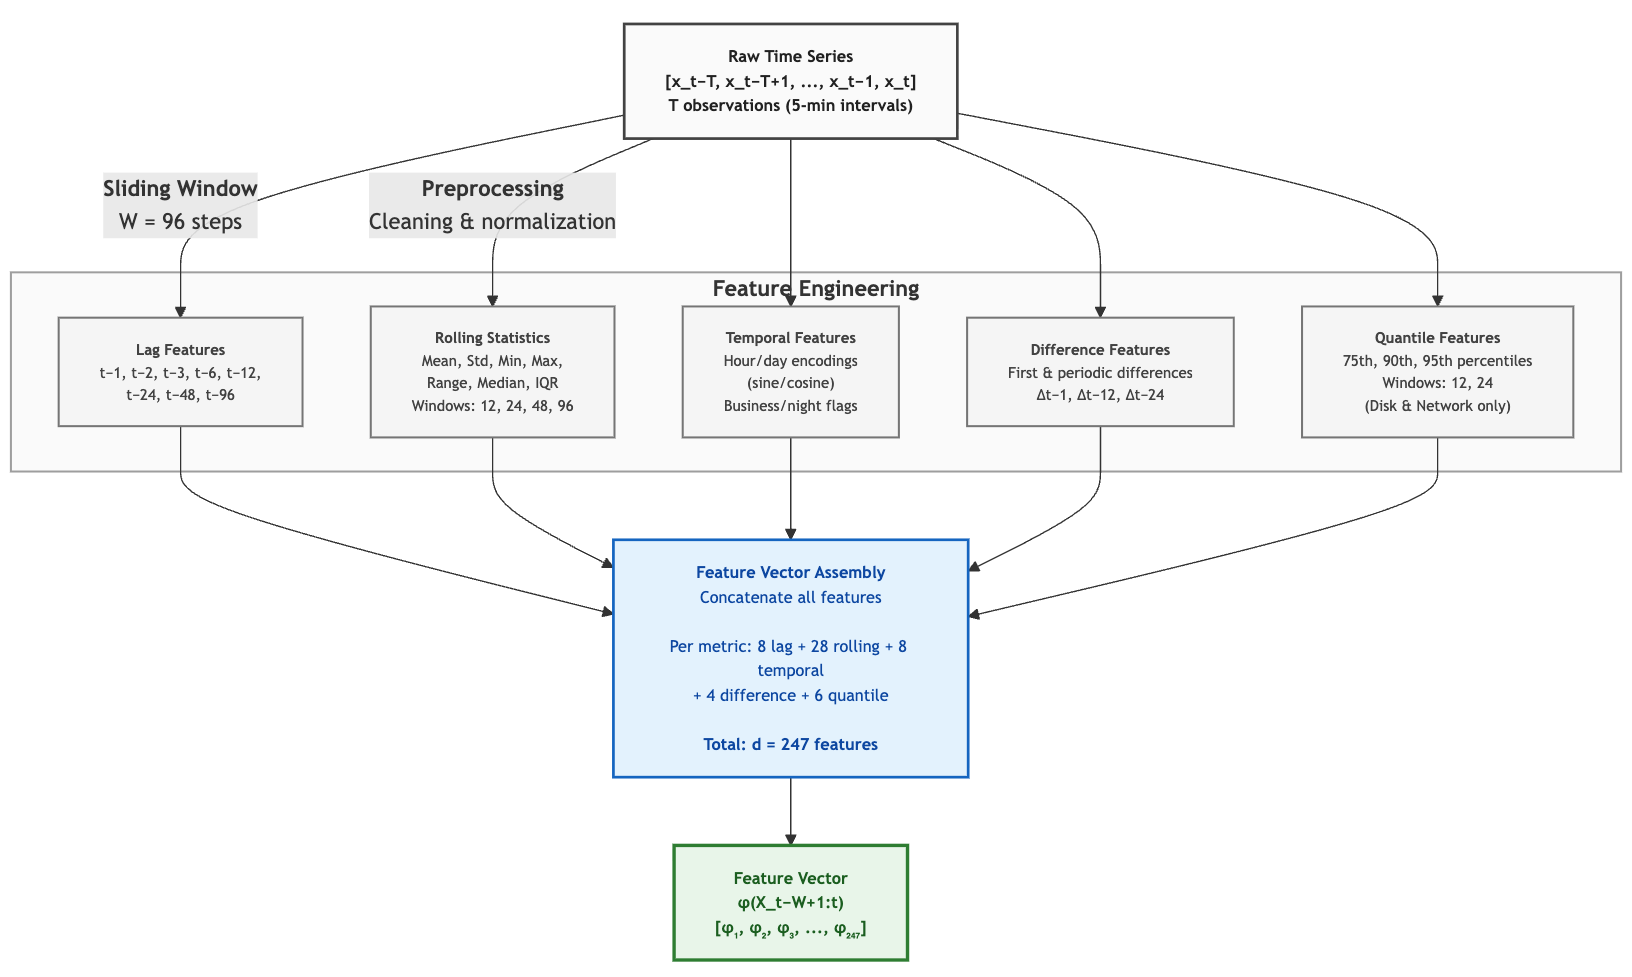
\includegraphics[width=\linewidth]{Feature-Engineering.png}
\caption{Overview of the preprocessing and feature engineering pipeline.}
\label{fig:feature_engineering}
\end{figure*}

Figure~\ref{fig:feature_engineering} illustrates the complete feature engineering pipeline. Starting from the cleaned sliding-window segment, we generate several complementary feature groups:

\begin{itemize}
    \item \textbf{Lag features:} Historical values at fixed offsets ($t-1, t-2, t-3, t-6, t-12, t-24, t-48, t-96$) that capture short-term autocorrelation and recent local dynamics.
    \item \textbf{Rolling statistics:} Aggregated statistics---mean, variance, min, max, range, median, and interquartile range---computed over multiple window sizes (12, 24, 48, 96 steps) to encode local context and variability.
    \item \textbf{Temporal features:} Diurnal and weekly encodings using sine/cosine transformations of hour and weekday, along with binary indicators for business hours and night periods.
    \item \textbf{Difference features:} First-order and periodic differences ($\Delta t = 1, 12, 24$) capturing momentum and phase-dependent variation.
    \item \textbf{Quantile features:} Upper-tail rolling percentiles (75th, 90th, 95th) for disk and network metrics, which exhibit bursty, heavy-tailed behavior.
\end{itemize}

These feature groups are concatenated into a unified representation $\phi(X_{t-W+1:t})$. Depending on the metric, a single prediction instance contains between 200 and 250 engineered features, with approximately $d=247$ features used in our configuration. This enriched representation captures both recent dynamics and structural patterns in the VM workload, enabling the downstream learning models to distinguish between steady-state behavior, short-term fluctuations, and burst events.

\subsection{Hybrid Tree-Based Model Architecture}
\label{subsec:hybrid_architecture}

The prediction stage employs a hybrid tree-based architecture in which the choice of model family is aligned with the statistical characteristics of each metric. CPU and memory usage exhibit relatively smooth trajectories with moderate variance and consistent short-term structure. Disk write throughput and network throughput, in contrast, display heavy-tailed distributions with abrupt bursts, outliers, and high temporal variability.

To accommodate these differences, we apply separate model families depending on the target metric:

\begin{itemize}
    \item \textbf{Random Forest (CPU and memory):}
    These metrics benefit from variance reduction through ensembling. We train Random Forest regressors composed of numerous decision trees built on bootstrap-resampled subsets of the data. Each tree explores different feature splits via random feature subsampling, enabling the ensemble to capture nonlinear dependencies while avoiding overfitting. Tree depth is limited to control complexity, and the final prediction is produced via averaging across all trees.

    \item \textbf{XGBoost (disk and network throughput):}
    These metrics exhibit burstiness and extreme skewness, making sequential gradient boosting more suitable. XGBoost fits trees iteratively to the current residuals, enabling the model to capture sharp deviations and high-order interactions. Regularization terms (L1/L2), learning rate control, and feature subsampling contribute to stable performance in the presence of noisy, high-variance data.
\end{itemize}

\begin{center}
\begin{minipage}{\columnwidth}
\centering
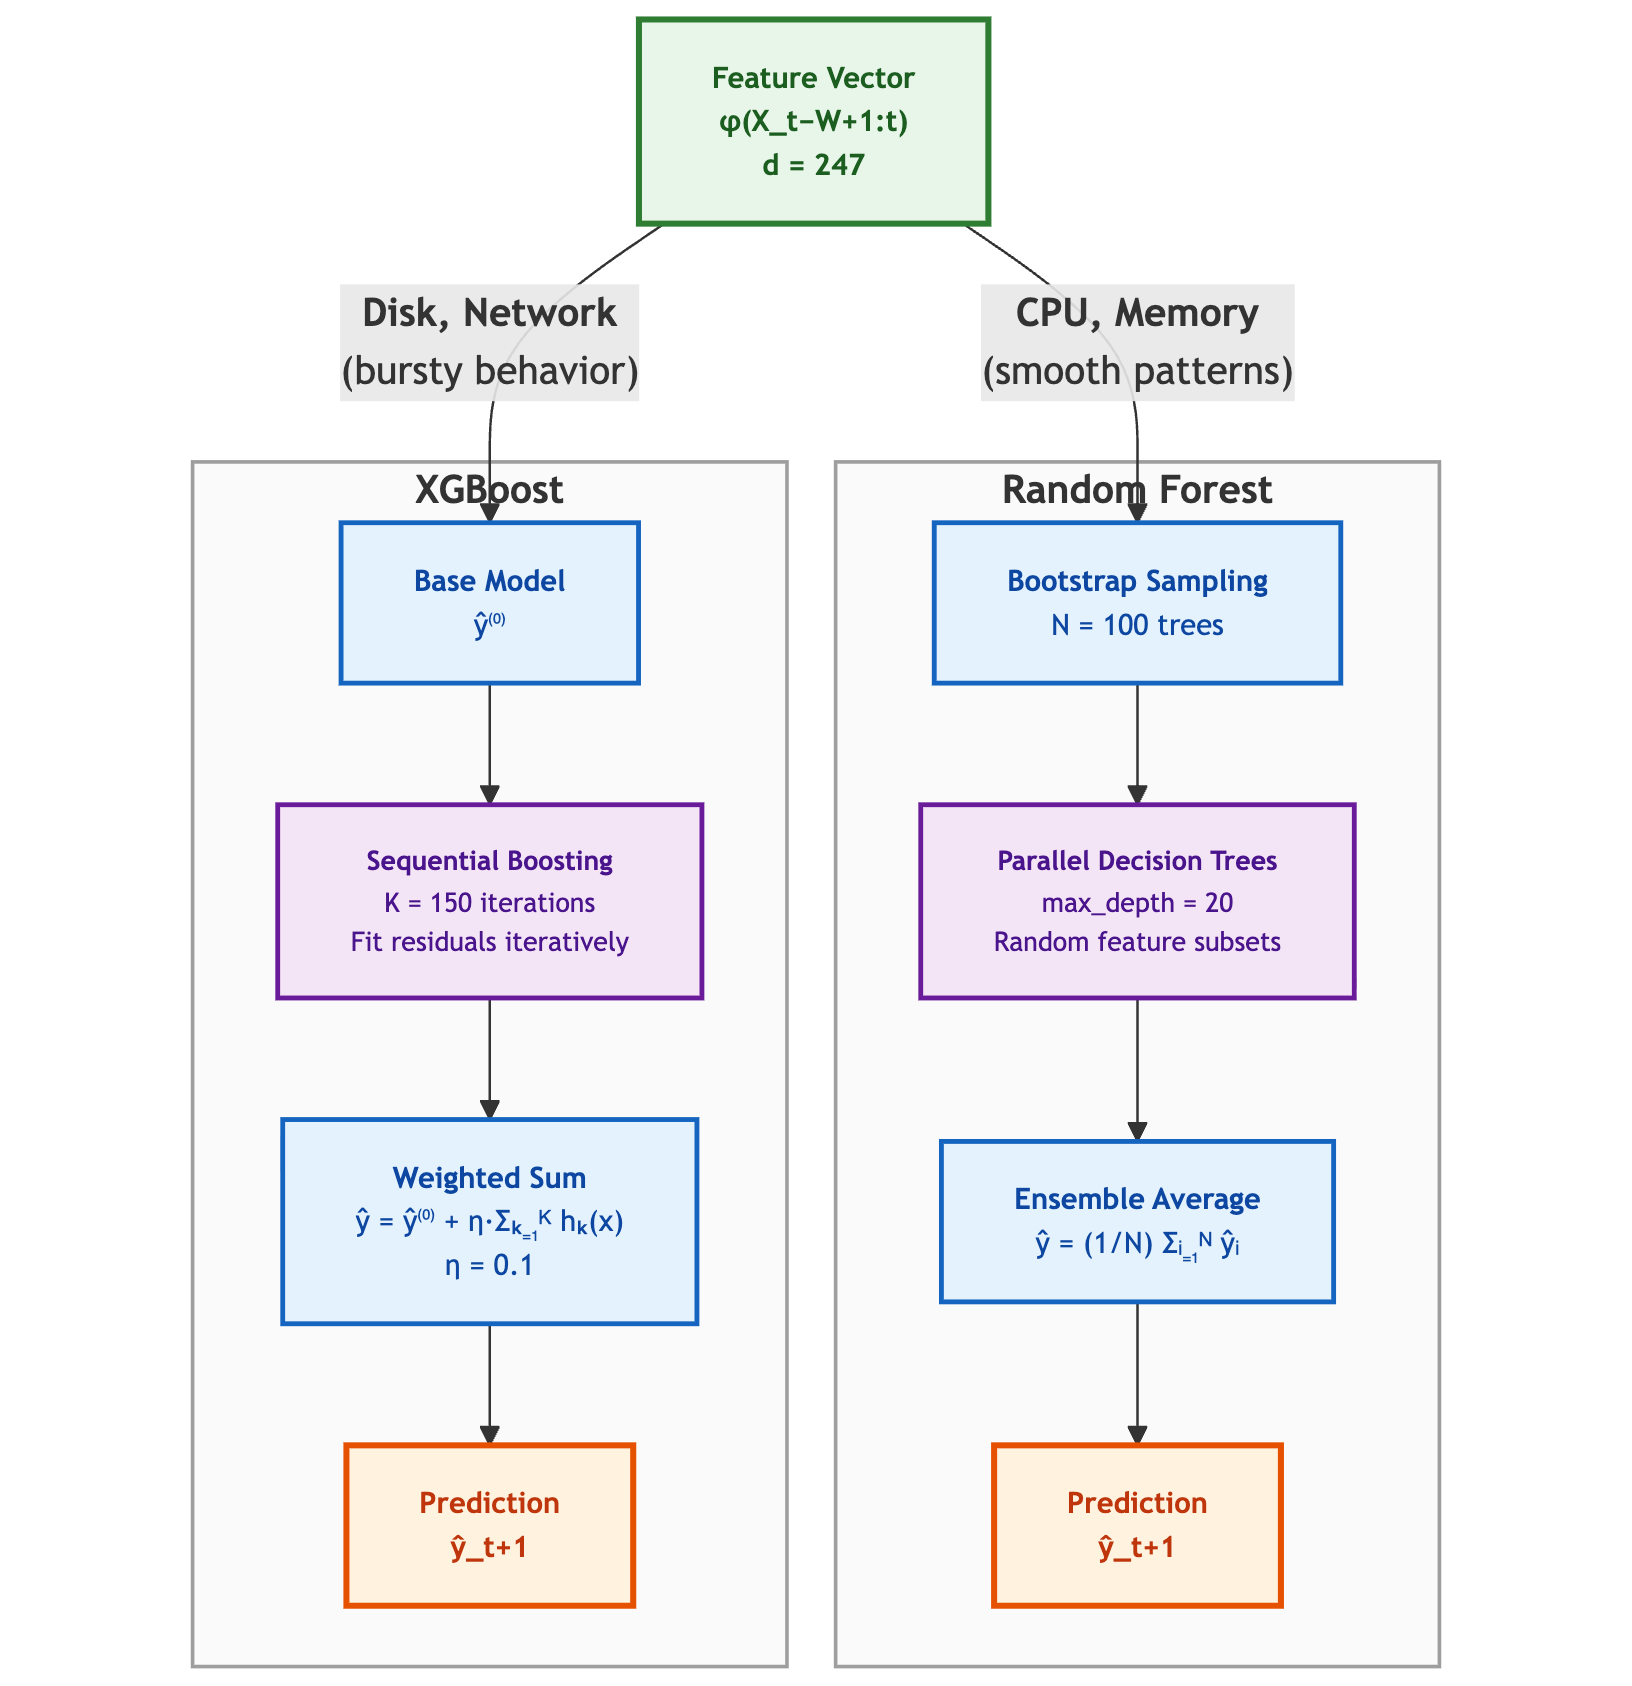
\includegraphics[width=\columnwidth]{Hybrid-based-approach.png}
\captionof{figure}{Hybrid tree-based modeling pipeline.}
\label{fig:hybrid_architecture}
\end{minipage}
\end{center}

Figure~\ref{fig:hybrid_architecture} presents the overall hybrid modeling workflow. The engineered feature vector $\phi(X_{t-W+1:t})$ serves as a common input to both models. For CPU and memory, the Random Forest aggregates predictions from parallel decision trees. For disk and network metrics, the XGBoost model applies sequential boosting to refine predictions through multiple iterations. This design ensures that each metric is modeled using an architecture consistent with its underlying statistical regime.

The output of each model is a one-step-ahead prediction $\hat{y}_{t+1}$ at VM granularity. This formulation enables real-time estimation of resource usage and performance behavior, forming a key component for SLA-driven, predictive CECC orchestration.

\subsection{Training and Evaluation Protocol}
\label{subsec:training}

Training and evaluation follow a time-aware protocol that reflects realistic deployment in CECC environments. For each VM and each target metric, the time series is split chronologically into three disjoint segments:
\begin{equation}
70\% \text{ training},\quad 15\% \text{ validation},\quad 15\% \text{ testing}.
\end{equation}

The training split is used to fit the model parameters, the validation split guides hyperparameter selection and early stopping, and the test split is reserved for final performance reporting. This chronological partition avoids leakage of future information into the training process and mimics an online prediction scenario where only past data are available at decision time.

Hyperparameters for the Random Forest and XGBoost models are chosen through a combination of grid search and manual refinement on the validation split, focusing on the number of estimators, maximum depth, and regularization parameters. For XGBoost, early stopping is applied using the validation loss to determine the effective number of boosting rounds. Once optimal configurations are identified, models are retrained on the combined training and validation data and evaluated on the held-out test segment.

We assess predictive performance using multiple complementary metrics. The primary accuracy measures are the coefficient of determination $R^2$, Mean Absolute Error (MAE), Root Mean Square Error (RMSE), and Mean Absolute Percentage Error (MAPE):

\begin{equation}
\text{MAE} = \frac{1}{N} \sum_{i=1}^{N} \big|y_i - \hat{y}_i\big|,
\end{equation}

\begin{equation}
\text{RMSE} = \sqrt{\frac{1}{N} \sum_{i=1}^{N} \big(y_i - \hat{y}_i\big)^2},
\end{equation}

\begin{equation}
R^2 = 1 - \frac{\sum_{i=1}^{N} \big(y_i - \hat{y}_i\big)^2}{\sum_{i=1}^{N} \big(y_i - \bar{y}\big)^2},
\end{equation}

\begin{equation}
\text{MAPE} = \frac{100}{N} \sum_{i=1}^{N} \left|\frac{y_i - \hat{y}_i}{y_i + \epsilon}\right|,
\end{equation}

where $y_i$ and $\hat{y}_i$ denote the true and predicted values, $\bar{y}$ is the mean of the true values, $N$ is the number of test samples, and $\epsilon$ is a small constant to avoid division by zero for near-zero targets. While MAE and RMSE quantify absolute error magnitudes, $R^2$ reflects the proportion of variance explained, and MAPE provides a scale-free measure of relative error that is informative for capacity planning and SLA thresholds.

Evaluation is performed independently for each of the four target metrics---CPU usage, memory usage, disk write throughput, and network throughput---across all three Materna traces. This per-metric, per-trace analysis allows us to quantify the robustness of the hybrid tree-based approach under diverse workload conditions and to identify metric-specific predictability patterns. The resulting scores and error distributions form the basis of the empirical study presented in the next section.

\section{Results and Discussion}
\label{sec:results}

This section evaluates the proposed hybrid tree-based framework on the GWA-T-13 Materna dataset, focusing on four key VM-level metrics: CPU usage, memory usage, disk write throughput, and network received/transmitted throughput. Table~\ref{tab:results} summarizes the quantitative performance of Random Forest and XGBoost models. The following narrative presents a detailed analysis for each metric together with representative figures, followed by an examination of feature importance, residual behavior, and overall generalization.

\begin{table*}[!t]
\centering
\caption{Prediction performance of tree-based models for VM resource metrics.}
\label{tab:results}
\setlength{\tabcolsep}{6pt}
\renewcommand{\arraystretch}{1.1}
\begin{tabular}{l l r r r r}
\hline
\textbf{Metric} & \textbf{Model} & \textbf{$R^2$} & \textbf{RMSE} & \textbf{MAE} & \textbf{MAPE (\%)} \\
\hline
CPU usage (\%)                    & RF       & 0.9416 & 0.17   & 0.10  &  3.7 \\
Memory usage (\%)                 & RF       & 0.8955 & 1.93   & 1.49  & 17.1 \\
Disk write throughput (KB/s)      & XGBoost  & 0.9568 & 12.62  & 0.86  &  4.1 \\
Network received throughput (KB/s)& XGBoost  & 0.9221 & 26.76  & 5.16  & 48.0 \\
Network transmitted throughput (KB/s)& XGBoost& 0.9071 & 30.87  & 8.68  &161.3 \\
\hline
\end{tabular}
\end{table*}

The Random Forest model performs strongly on CPU usage, achieving $R^2 \approx 0.94$ with very low error. CPU dynamics in this enterprise workload exhibit relatively smooth fluctuations with occasional spikes, making them well suited to variance-reducing ensembles. Figure~\ref{fig:cpu_rf_results} shows the full prediction horizon, a zoomed view, and the corresponding scatter plot. The close alignment between predicted and actual values confirms that short-term variations are effectively captured, aided by lag-based and rolling-window features that encode recent CPU behavior.

\begin{center}
\begin{minipage}{\columnwidth}
\centering
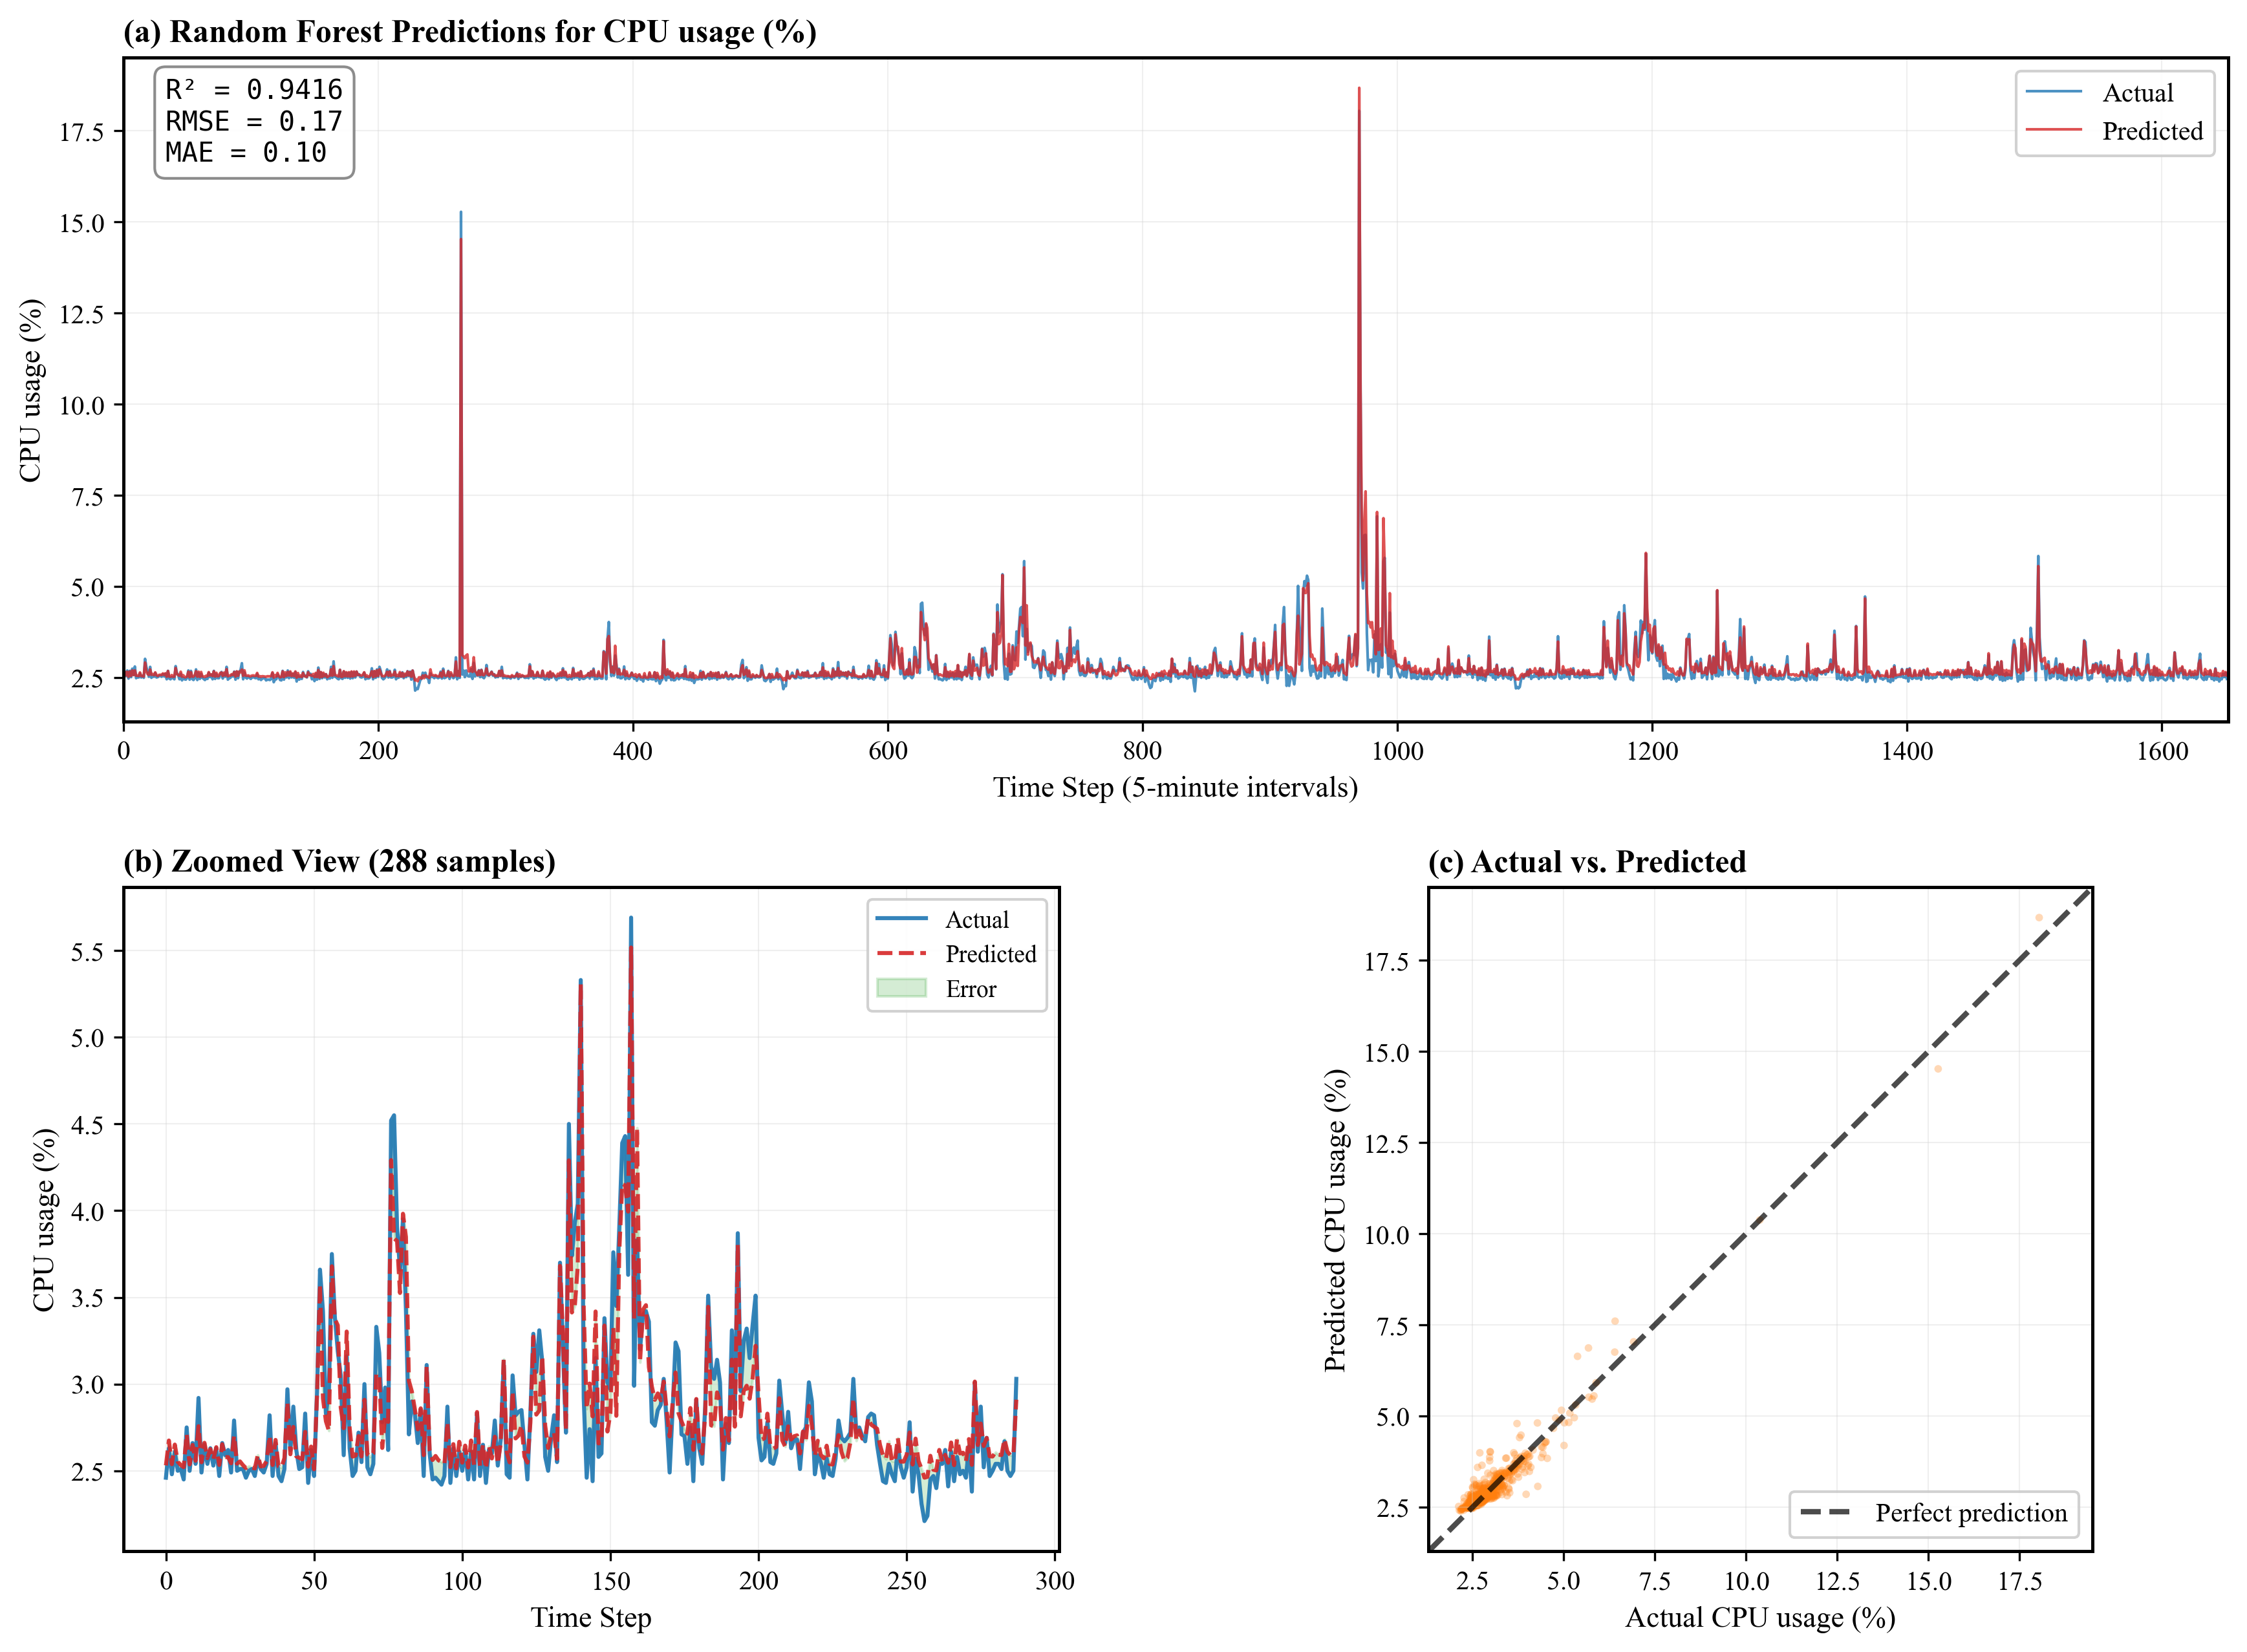
\includegraphics[width=\columnwidth]{figure_CPU_usage_pct}
\captionof{figure}{Random Forest predictions for CPU usage: (a) full-sequence prediction, (b) zoomed view, (c) actual vs.\ predicted scatter.}
\label{fig:cpu_rf_results}
\end{minipage}
\end{center}

Memory usage exhibits greater variability and faster transitions than CPU, yet the Random Forest still achieves $R^2 \approx 0.89$. The model effectively captures both baseline levels and abrupt changes, as shown in Figure~\ref{fig:mem_rf_results}. Medium-horizon rolling features play a central role in representing the working-set memory patterns typical of enterprise workloads. Deviations primarily occur during rapid allocation/deallocation phases, but these are short lived and do not accumulate over time.

\begin{center}
\begin{minipage}{\columnwidth}
\centering
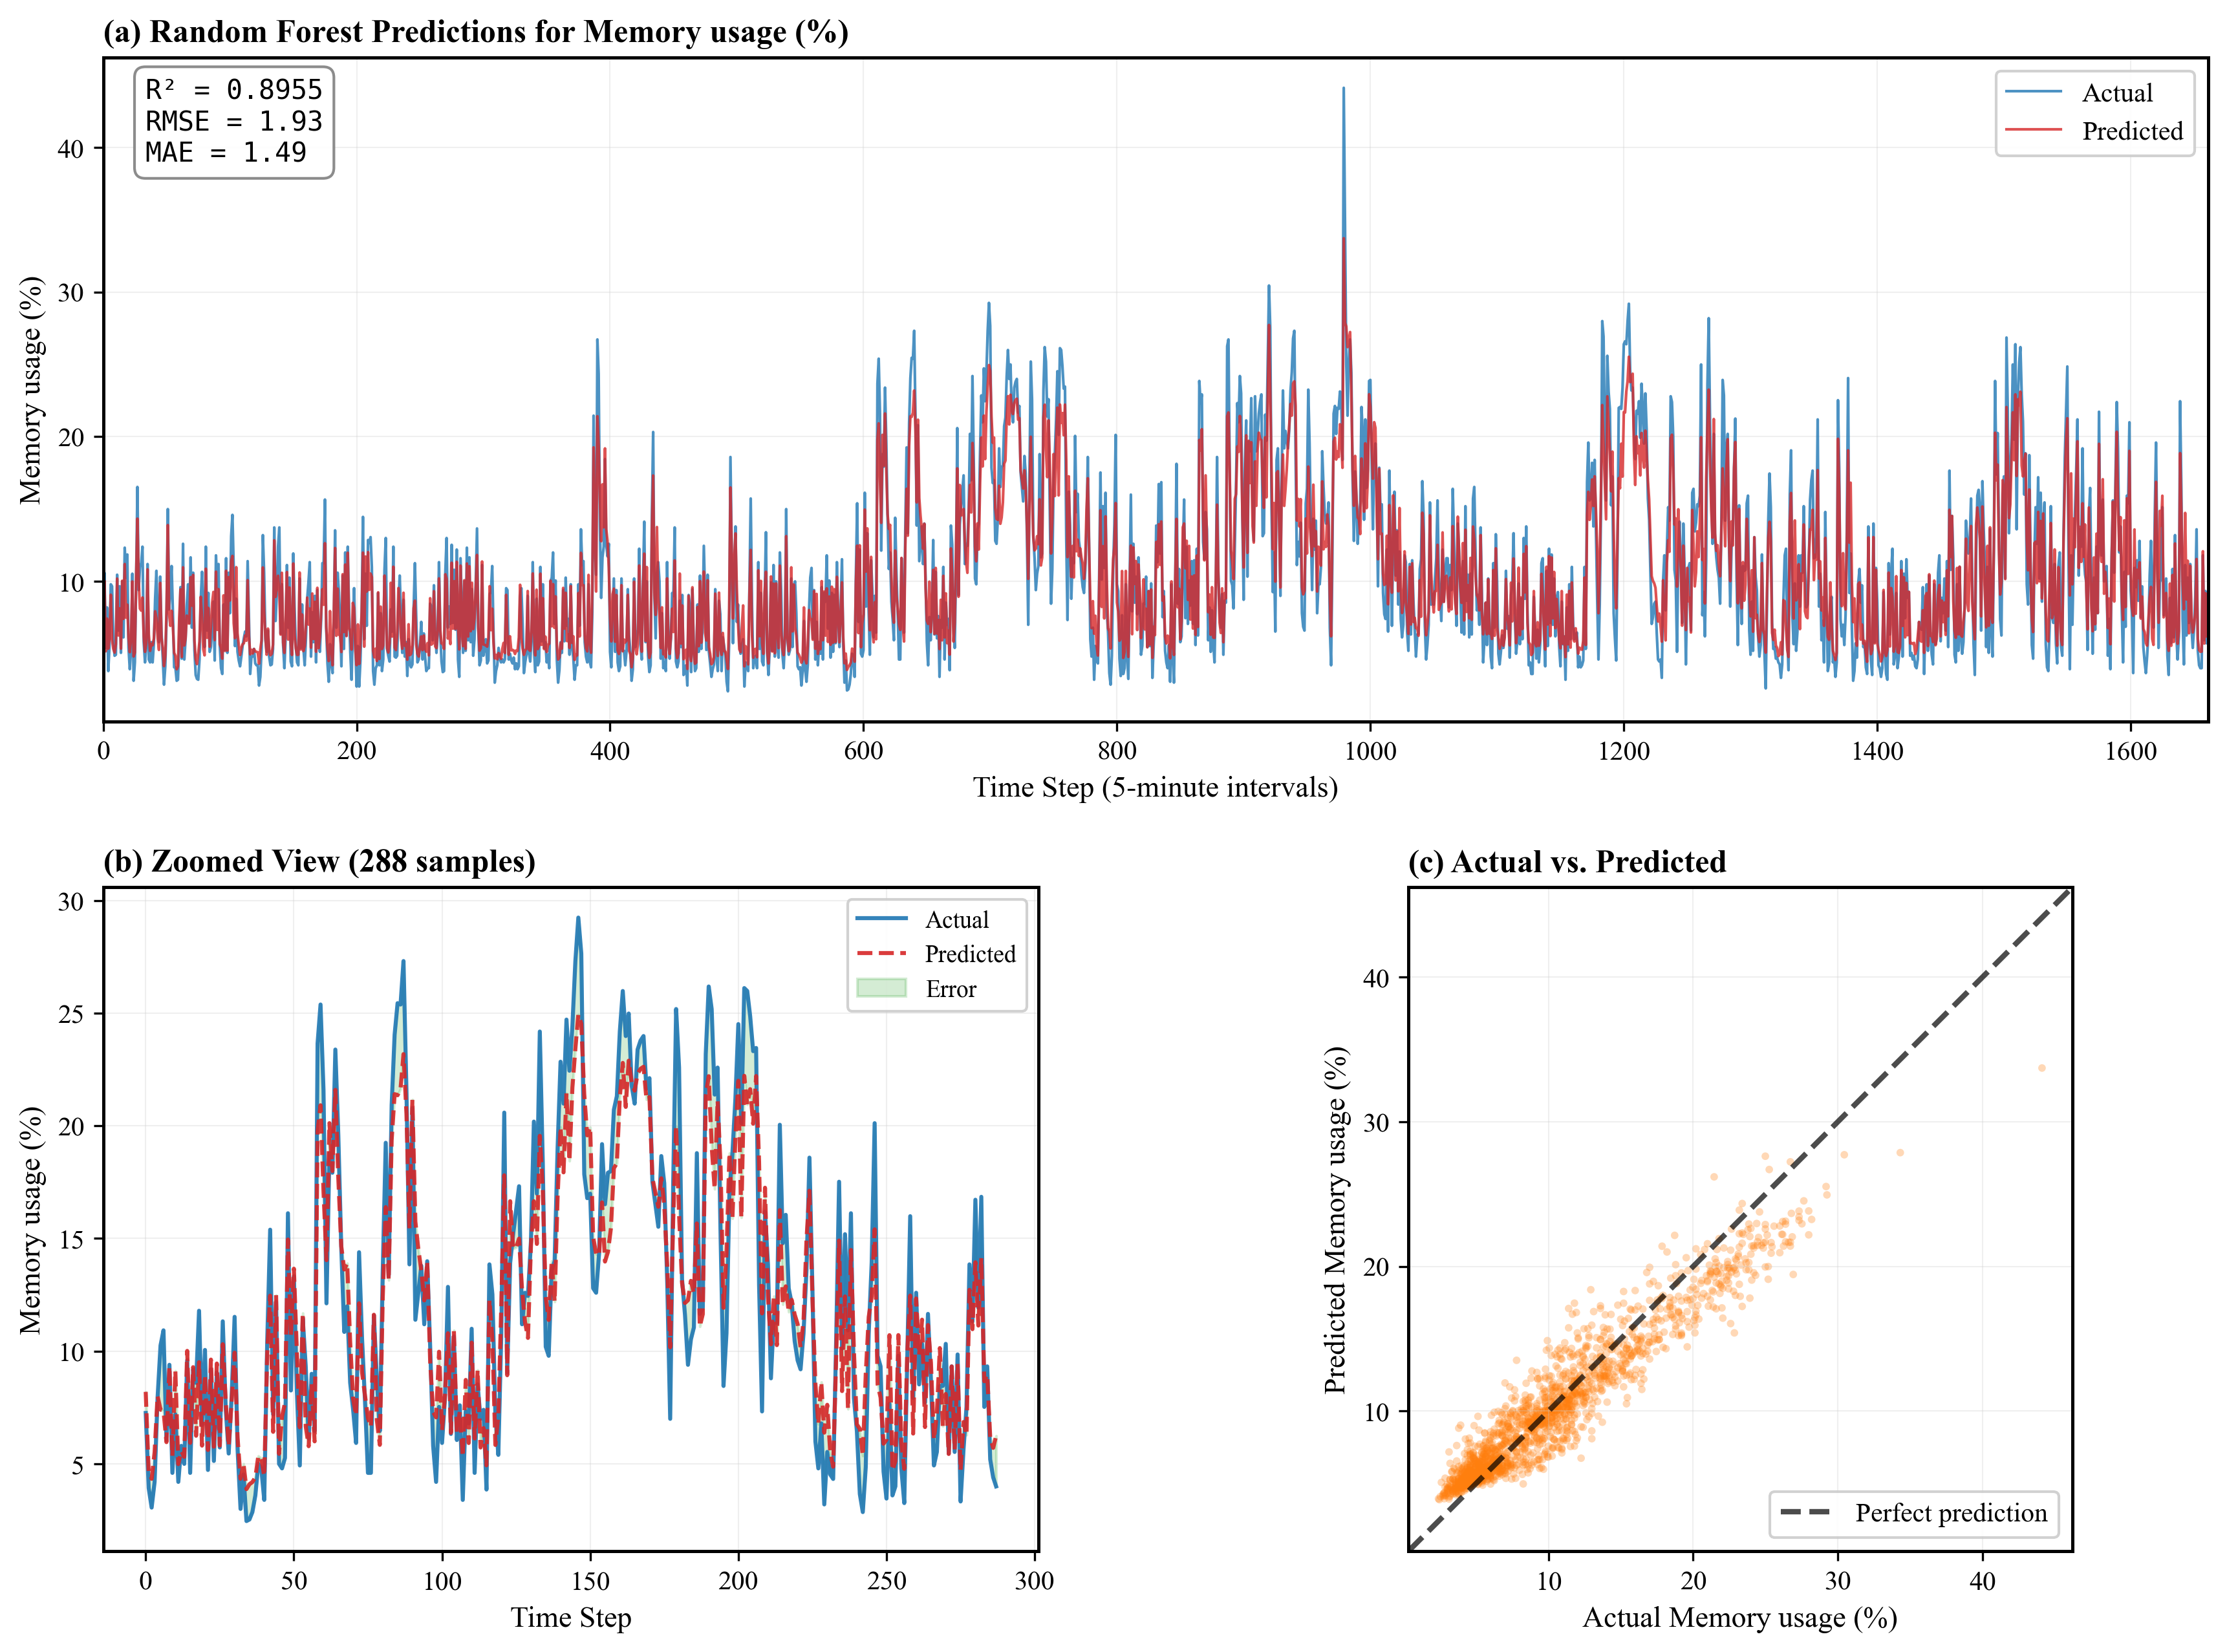
\includegraphics[width=\columnwidth]{figure_Memory_usage_pct.png}
\captionof{figure}{Random Forest predictions for memory usage: (a) full-sequence prediction, (b) zoomed view, (c) actual vs.\ predicted scatter.}
\label{fig:mem_rf_results}
\end{minipage}
\end{center}

Disk write throughput displays heavy-tailed behavior and extreme skewness, with intermittent bursts reaching several orders of magnitude above idle values. XGBoost performs exceptionally well under these conditions ($R^2 \approx 0.96$), as shown in Figure~\ref{fig:disk_xgb_results}. Its sequential error-correcting boosting mechanism enables it to model rare but high-impact spikes while avoiding overfitting through regularization. Long-window rolling maxima and quantile-based features, which summarize burst intensity and recency, are key to achieving predictive stability for this metric.

\begin{center}
\begin{minipage}{\columnwidth}
\centering
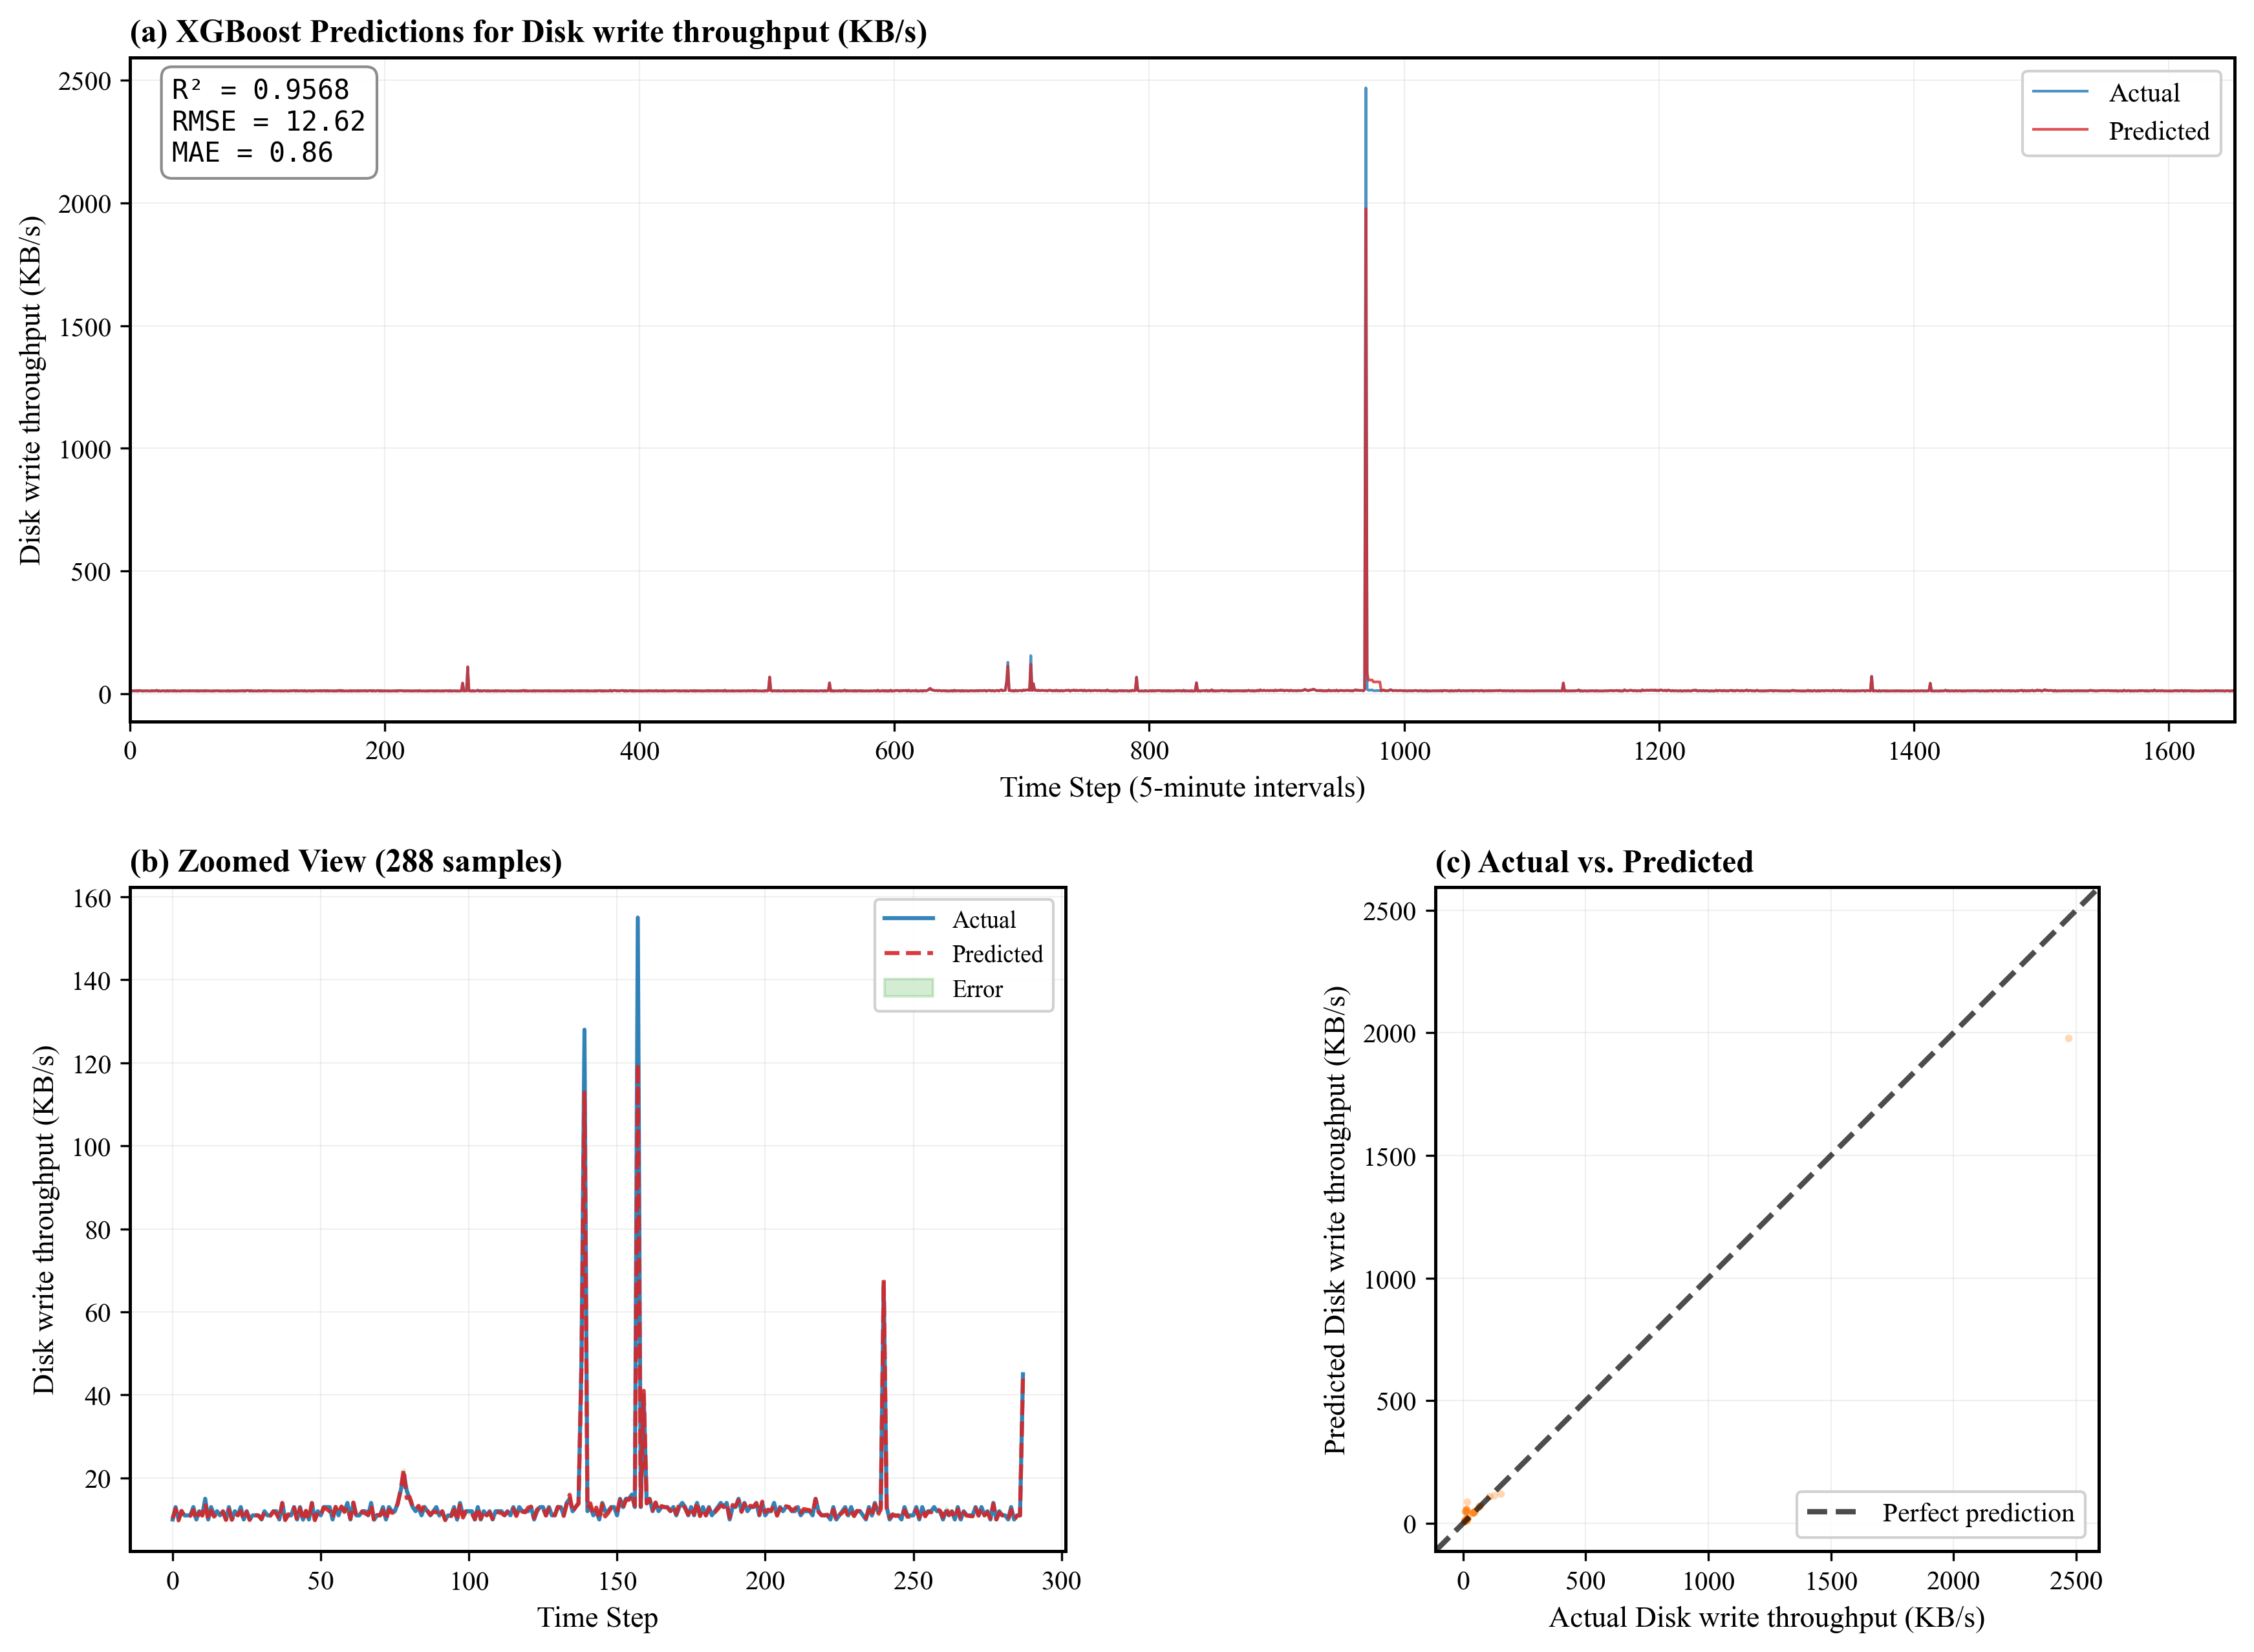
\includegraphics[width=\columnwidth]{figure_Disk_write_throughput_KB_s.png}
\captionof{figure}{XGBoost predictions for disk write throughput: (a) full-sequence prediction, (b) zoomed view, (c) actual vs.\ predicted scatter.}
\label{fig:disk_rf_results}
\end{minipage}
\end{center}

Network received throughput also exhibits bursty, long-tailed dynamics. The XGBoost model achieves $R^2 \approx 0.92$, balancing accurate modeling of low-utilization regions with reasonable handling of extreme outliers. Figure~\ref{fig:netrx_xgb_results} shows that peaks are sometimes underestimated in magnitude---an expected trade-off in heavy-tailed distributions---but their timing and relative scale remain well predicted, which is crucial for proactive CECC orchestration and congestion avoidance.

\begin{center}
\begin{minipage}{\columnwidth}
\centering
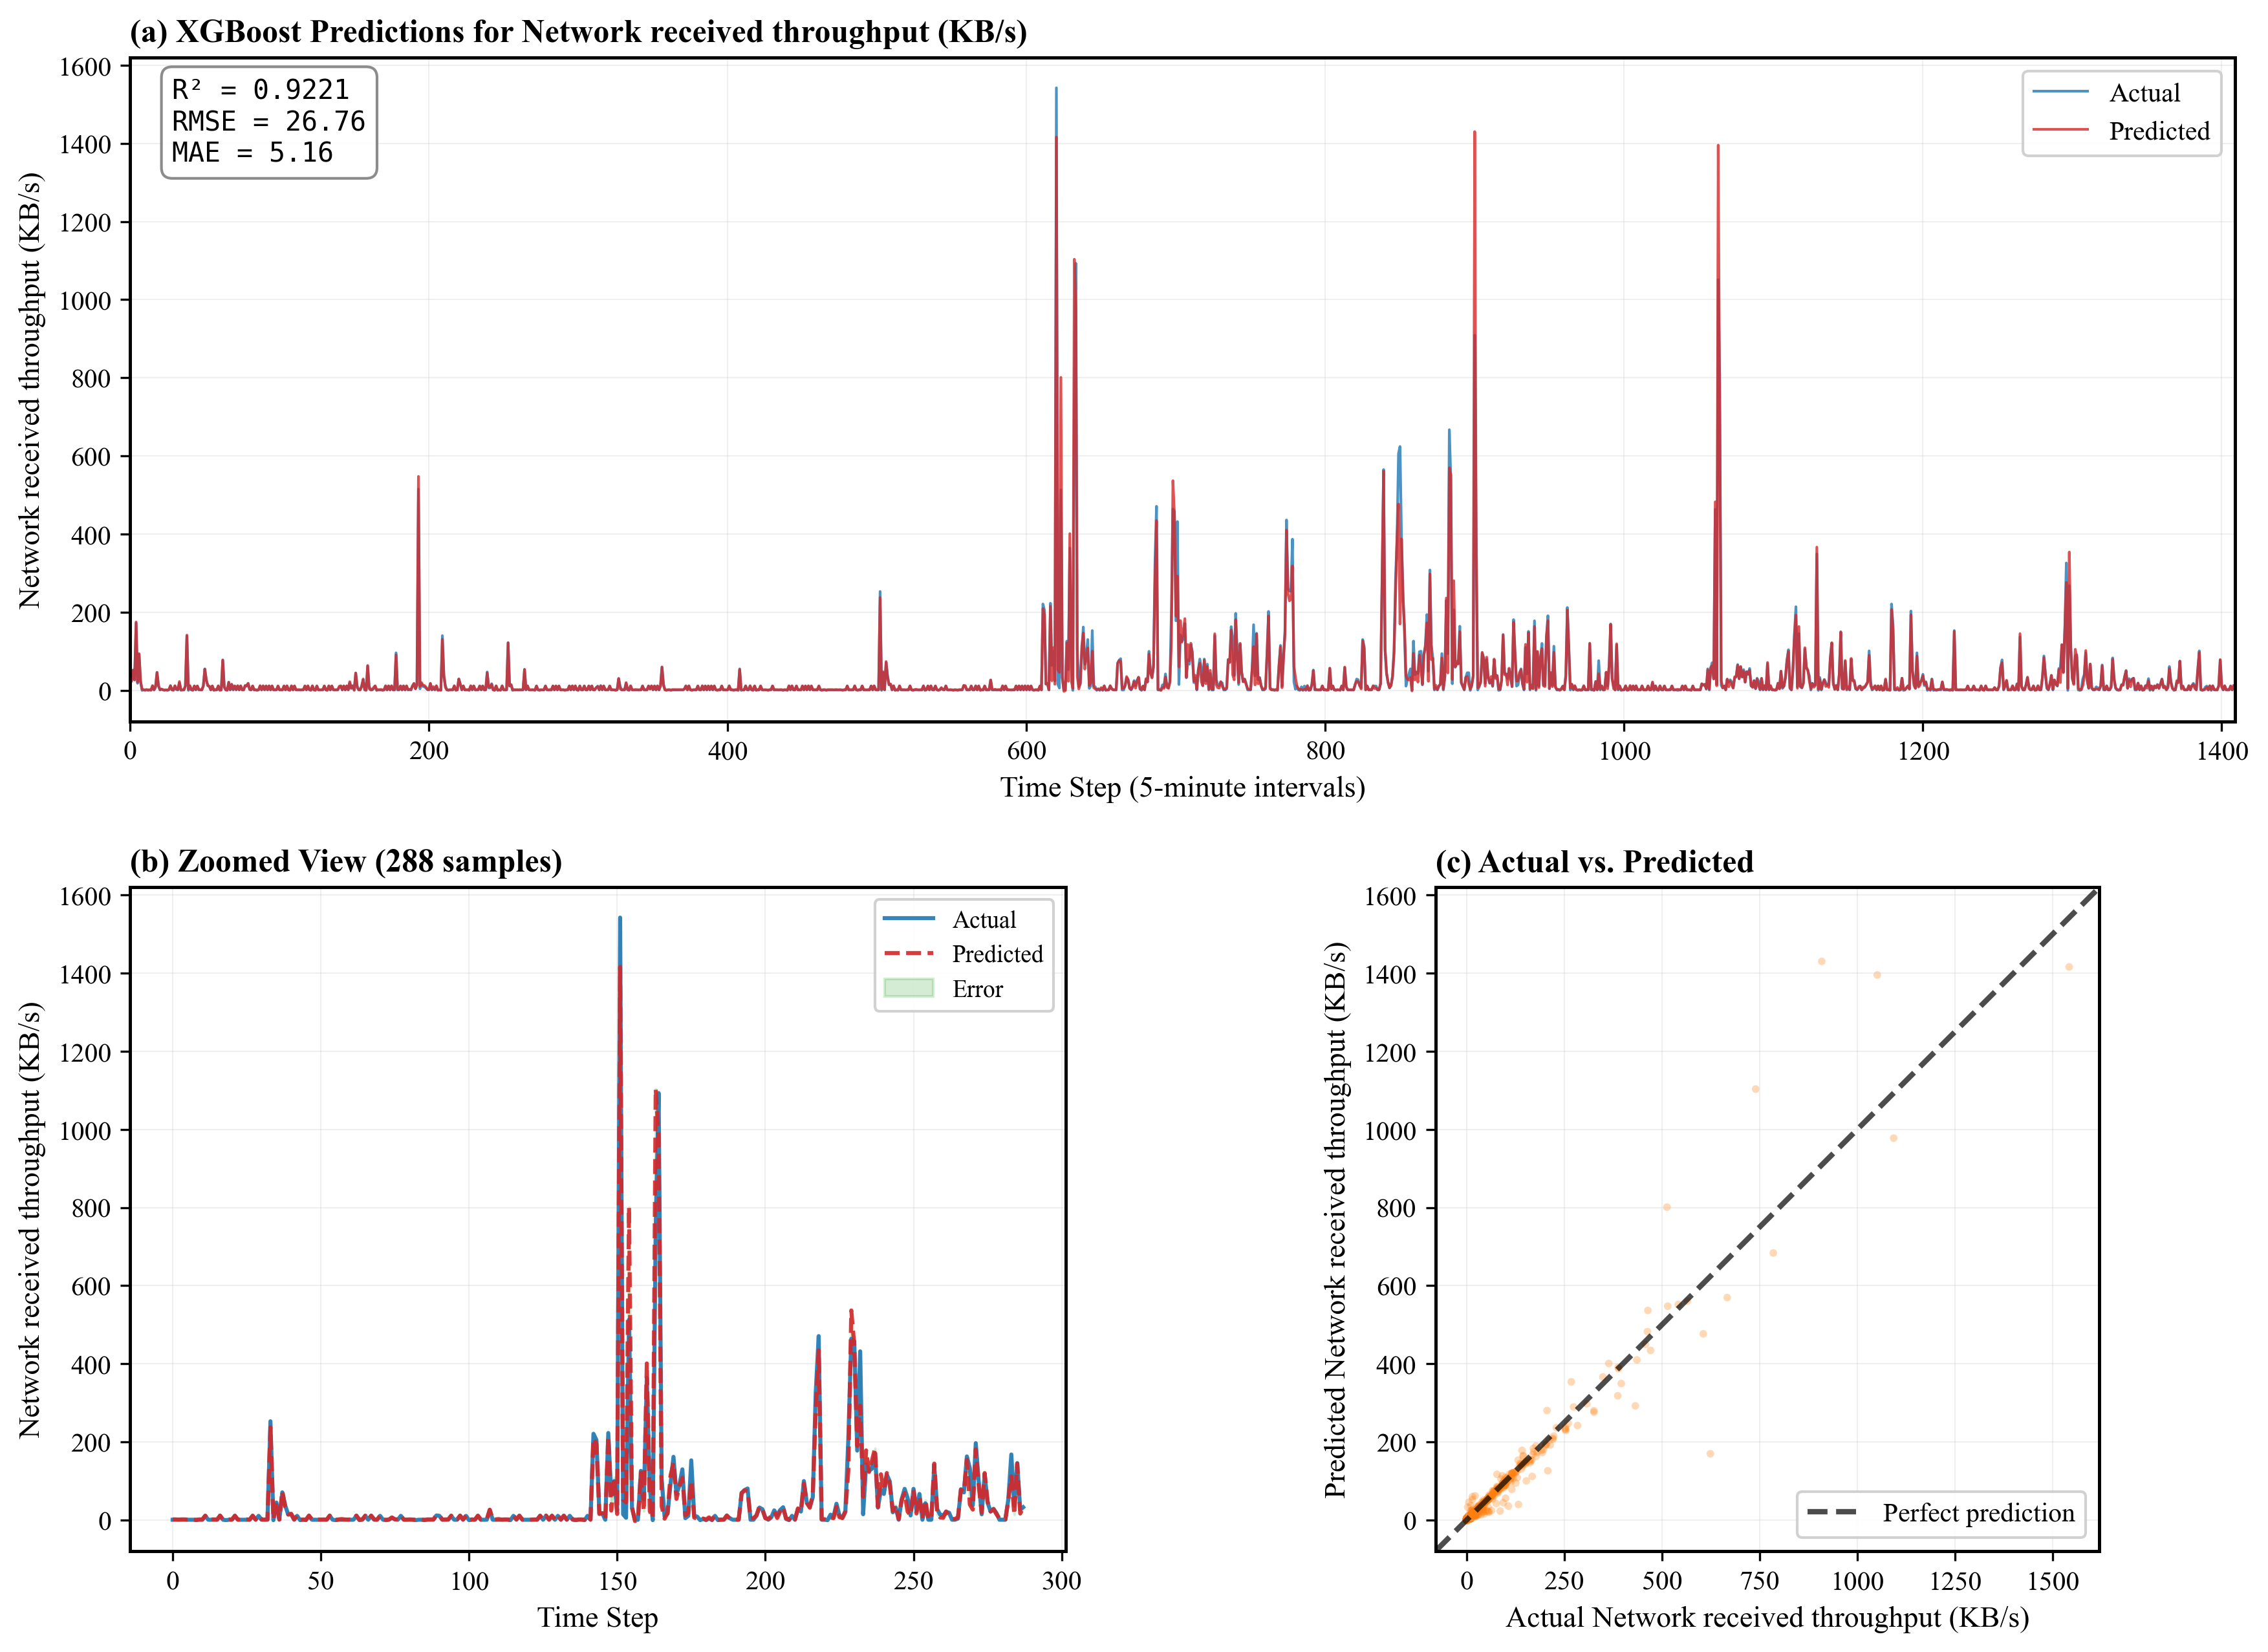
\includegraphics[width=\columnwidth]{figure_Network_received_throughput_KB_s.png}
\captionof{figure}{XGBoost predictions for network received throughput: (a) full-sequence prediction, (b) zoomed view, (c) actual vs.\ predicted scatter.}
\label{fig:netrx_rf_results}
\end{minipage}
\end{center}


Network transmitted throughput exhibits the strongest extreme spikes among all metrics. Despite this challenge, XGBoost attains $R^2 \approx 0.91$ and captures both baseline behavior and moderate bursts effectively, as illustrated in Figure~\ref{fig:nettx_xgb_results}. Prediction errors concentrate around the most extreme outliers, yet overall residual patterns remain stable, with no systematic bias or drift over time, indicating that the model generalizes well across different operating regimes.

\begin{center}
\begin{minipage}{\columnwidth}
\centering
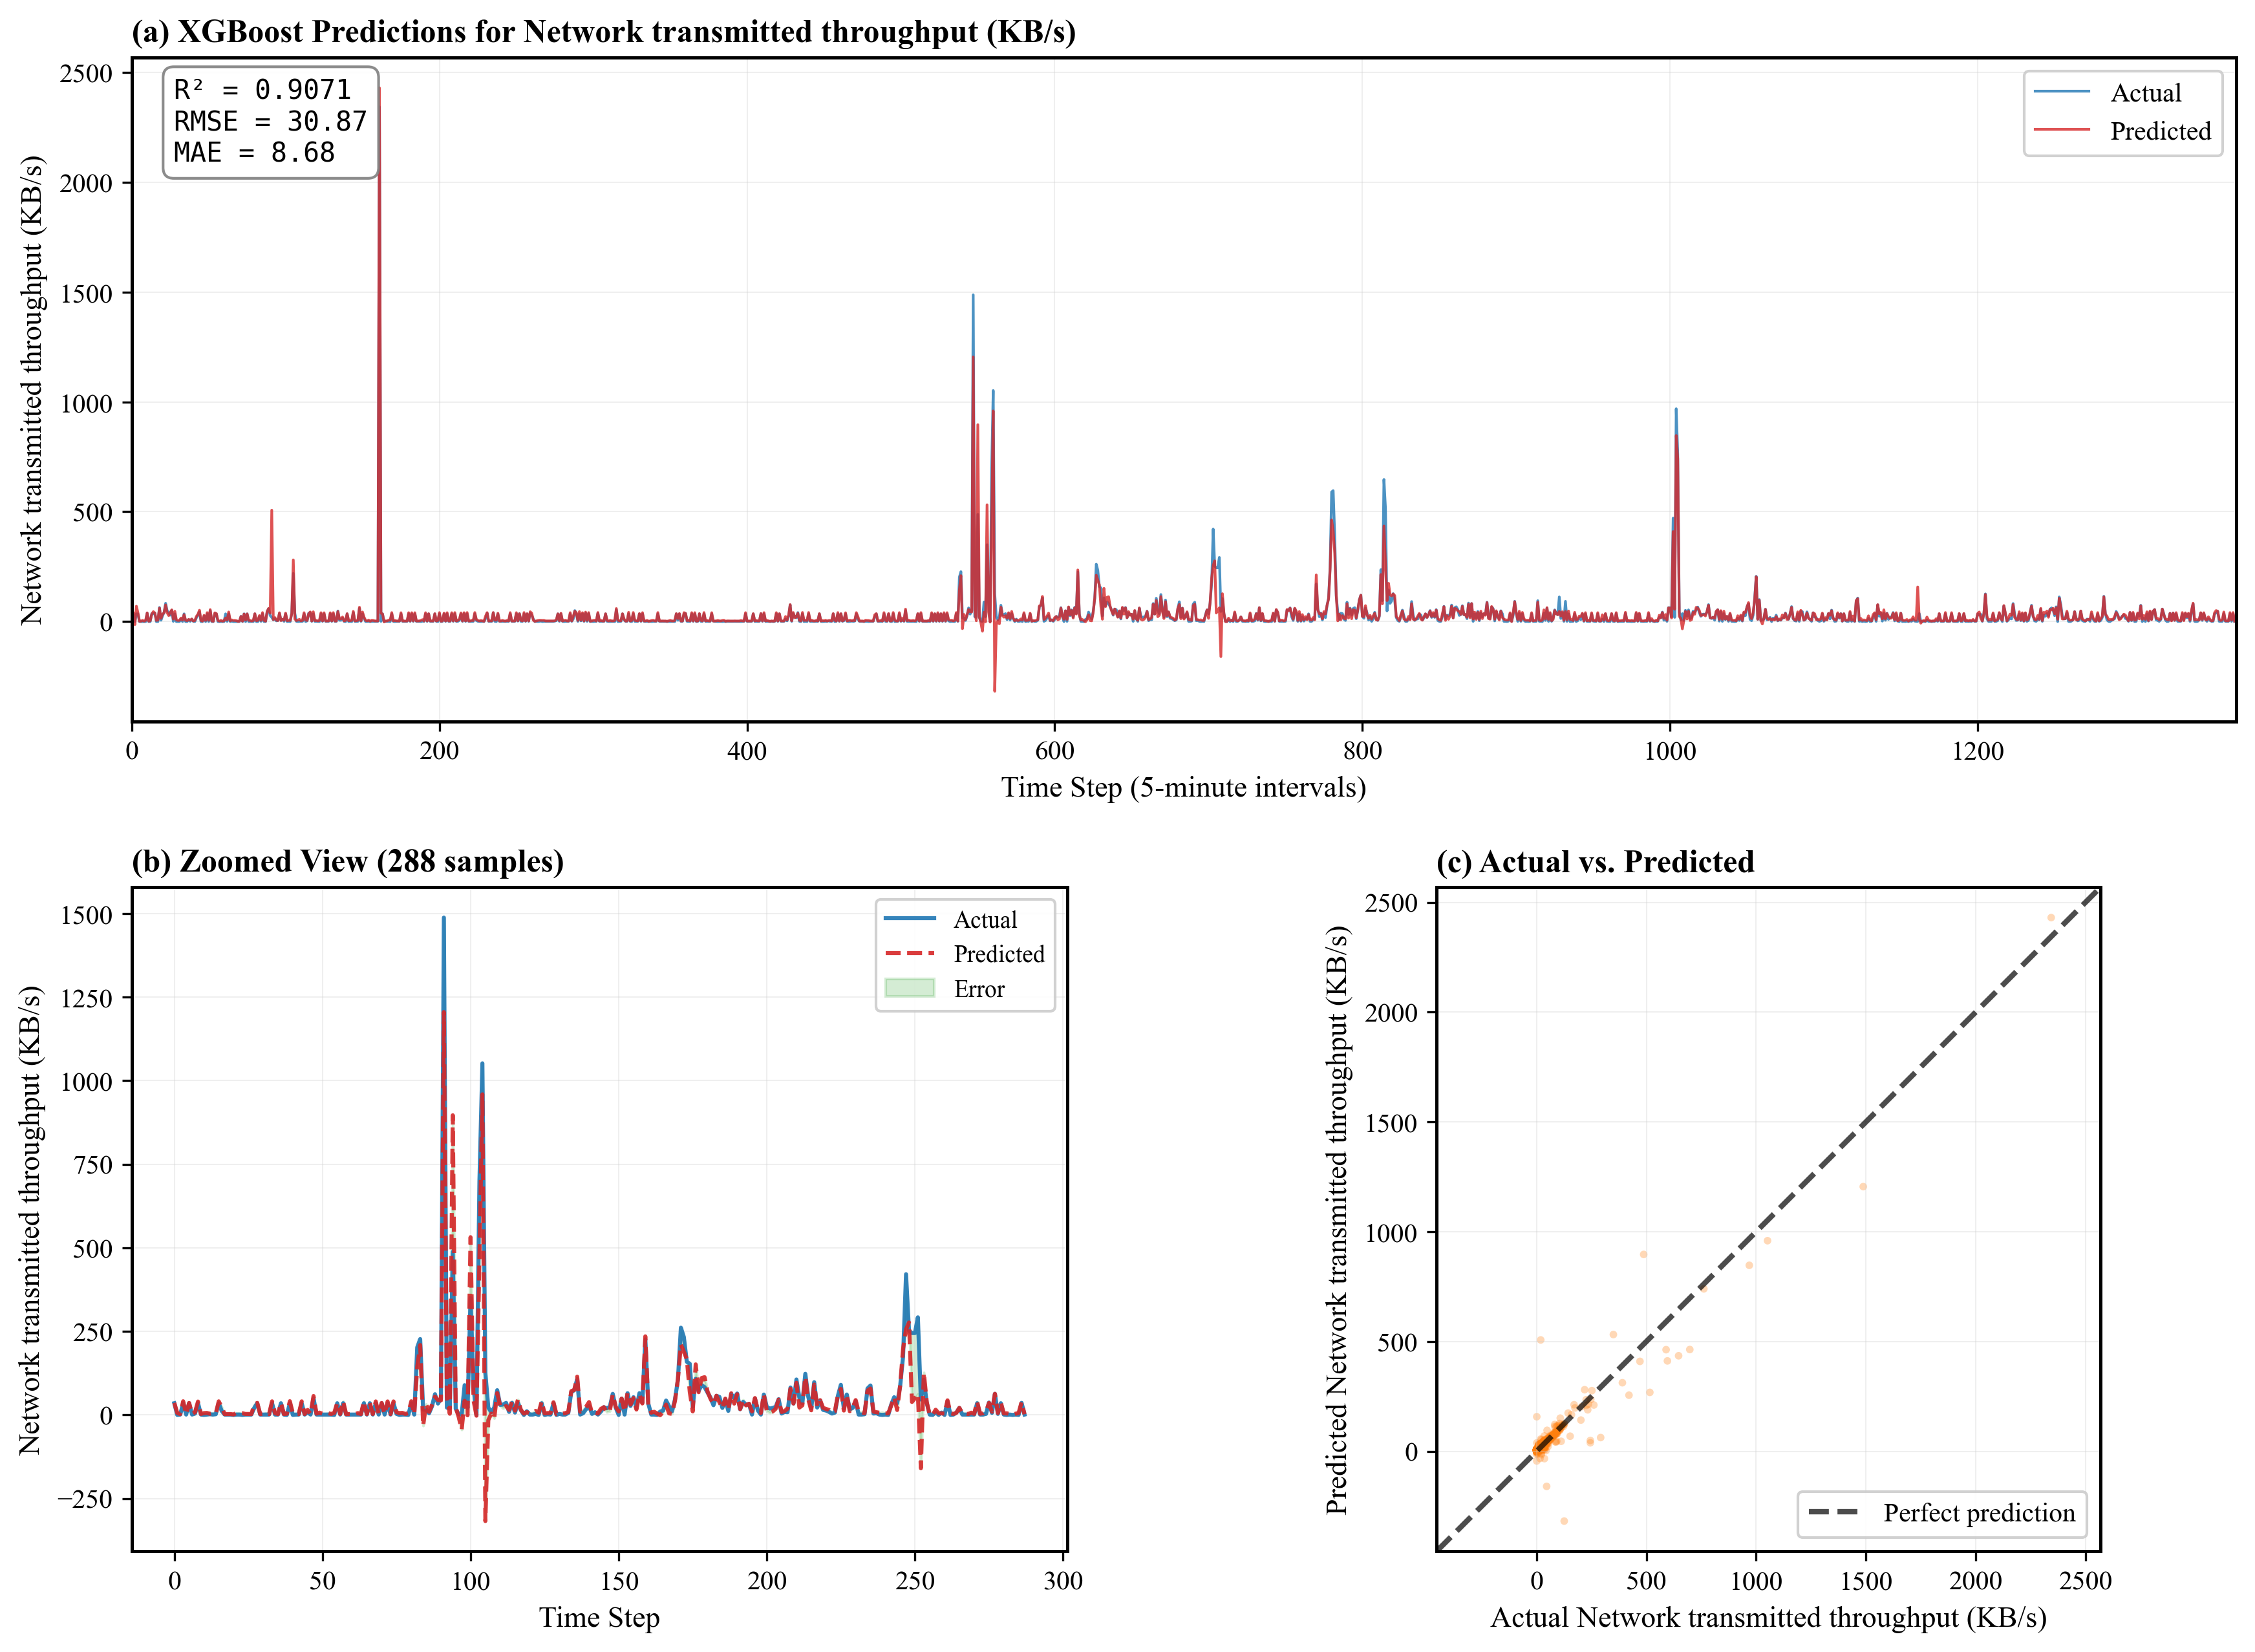
\includegraphics[width=\columnwidth]{figure_Network_transmitted_throughput_KB_s.png}
\captionof{figure}{XGBoost predictions for network transmitted throughput: (a) full-sequence prediction, (b) zoomed view, (c) actual vs.\ predicted scatter.}
\label{fig:nettx_rf_results}
\end{minipage}
\end{center}


Compared to these tree-based models, LSTM architectures delivered consistently lower accuracy in this setting. The resource traces exhibit non-stationarity, heavy-tailed distributions, and irregular burstiness, making it difficult for sequence models relying on smooth temporal dependencies to learn effectively. Short-horizon forecasting further favors explicit feature engineering over implicit temporal representation learning. Additionally, LSTMs are sensitive to scaling and hyperparameter configurations, which complicates their deployment for multi-metric, per-VM prediction. In contrast, tree-based models leverage engineered lag, rolling, and temporal features directly, enabling strong generalization with comparatively lower training complexity.

Residual analysis across metrics reveals consistent patterns. For CPU and memory, residuals remain small and stable throughout the trace, with no visible temporal correlation beyond short-lived local fluctuations. For disk and network metrics, residuals cluster tightly around zero in low-activity regimes and widen during rare bursts, reflecting the inherent imbalance between bulk and extreme values. Importantly, no systematic error drift is observed, and predictions remain robust across different time periods, indicating stable generalization over the month-long dataset.

Feature-importance profiles confirm the central role of engineered temporal features. Short-lag features dominate across all metrics, capturing immediate autocorrelation and recent trends. Rolling statistics (mean, range, variance) over multi-hour windows play a major role for CPU and memory, reflecting gradual utilization cycles. Disk and network prediction is driven by long-window maxima, quantiles, and dispersion measures, which encode burstiness and variability. Cyclical time-of-day and day-of-week features also contribute significantly, particularly for CPU, due to strong periodic usage patterns in enterprise workloads.

The combined view in Figure~\ref{fig:summary_results} highlights the complementary strengths of Random Forest and XGBoost. No single model family can optimally capture the distinct statistical characteristics of CPU, memory, disk I/O, and network I/O. The hybrid design therefore provides a principled, scalable, and interpretable solution for short-term, per-VM application performance prediction in CECC environments. By exploiting the strengths of Random Forest on smoother CPU and memory trajectories and the robustness of XGBoost on bursty disk and network metrics, the framework delivers high predictive accuracy while remaining computationally efficient and amenable to parallel training across many VMs.

\begin{center}
\begin{minipage}{\columnwidth}
\centering
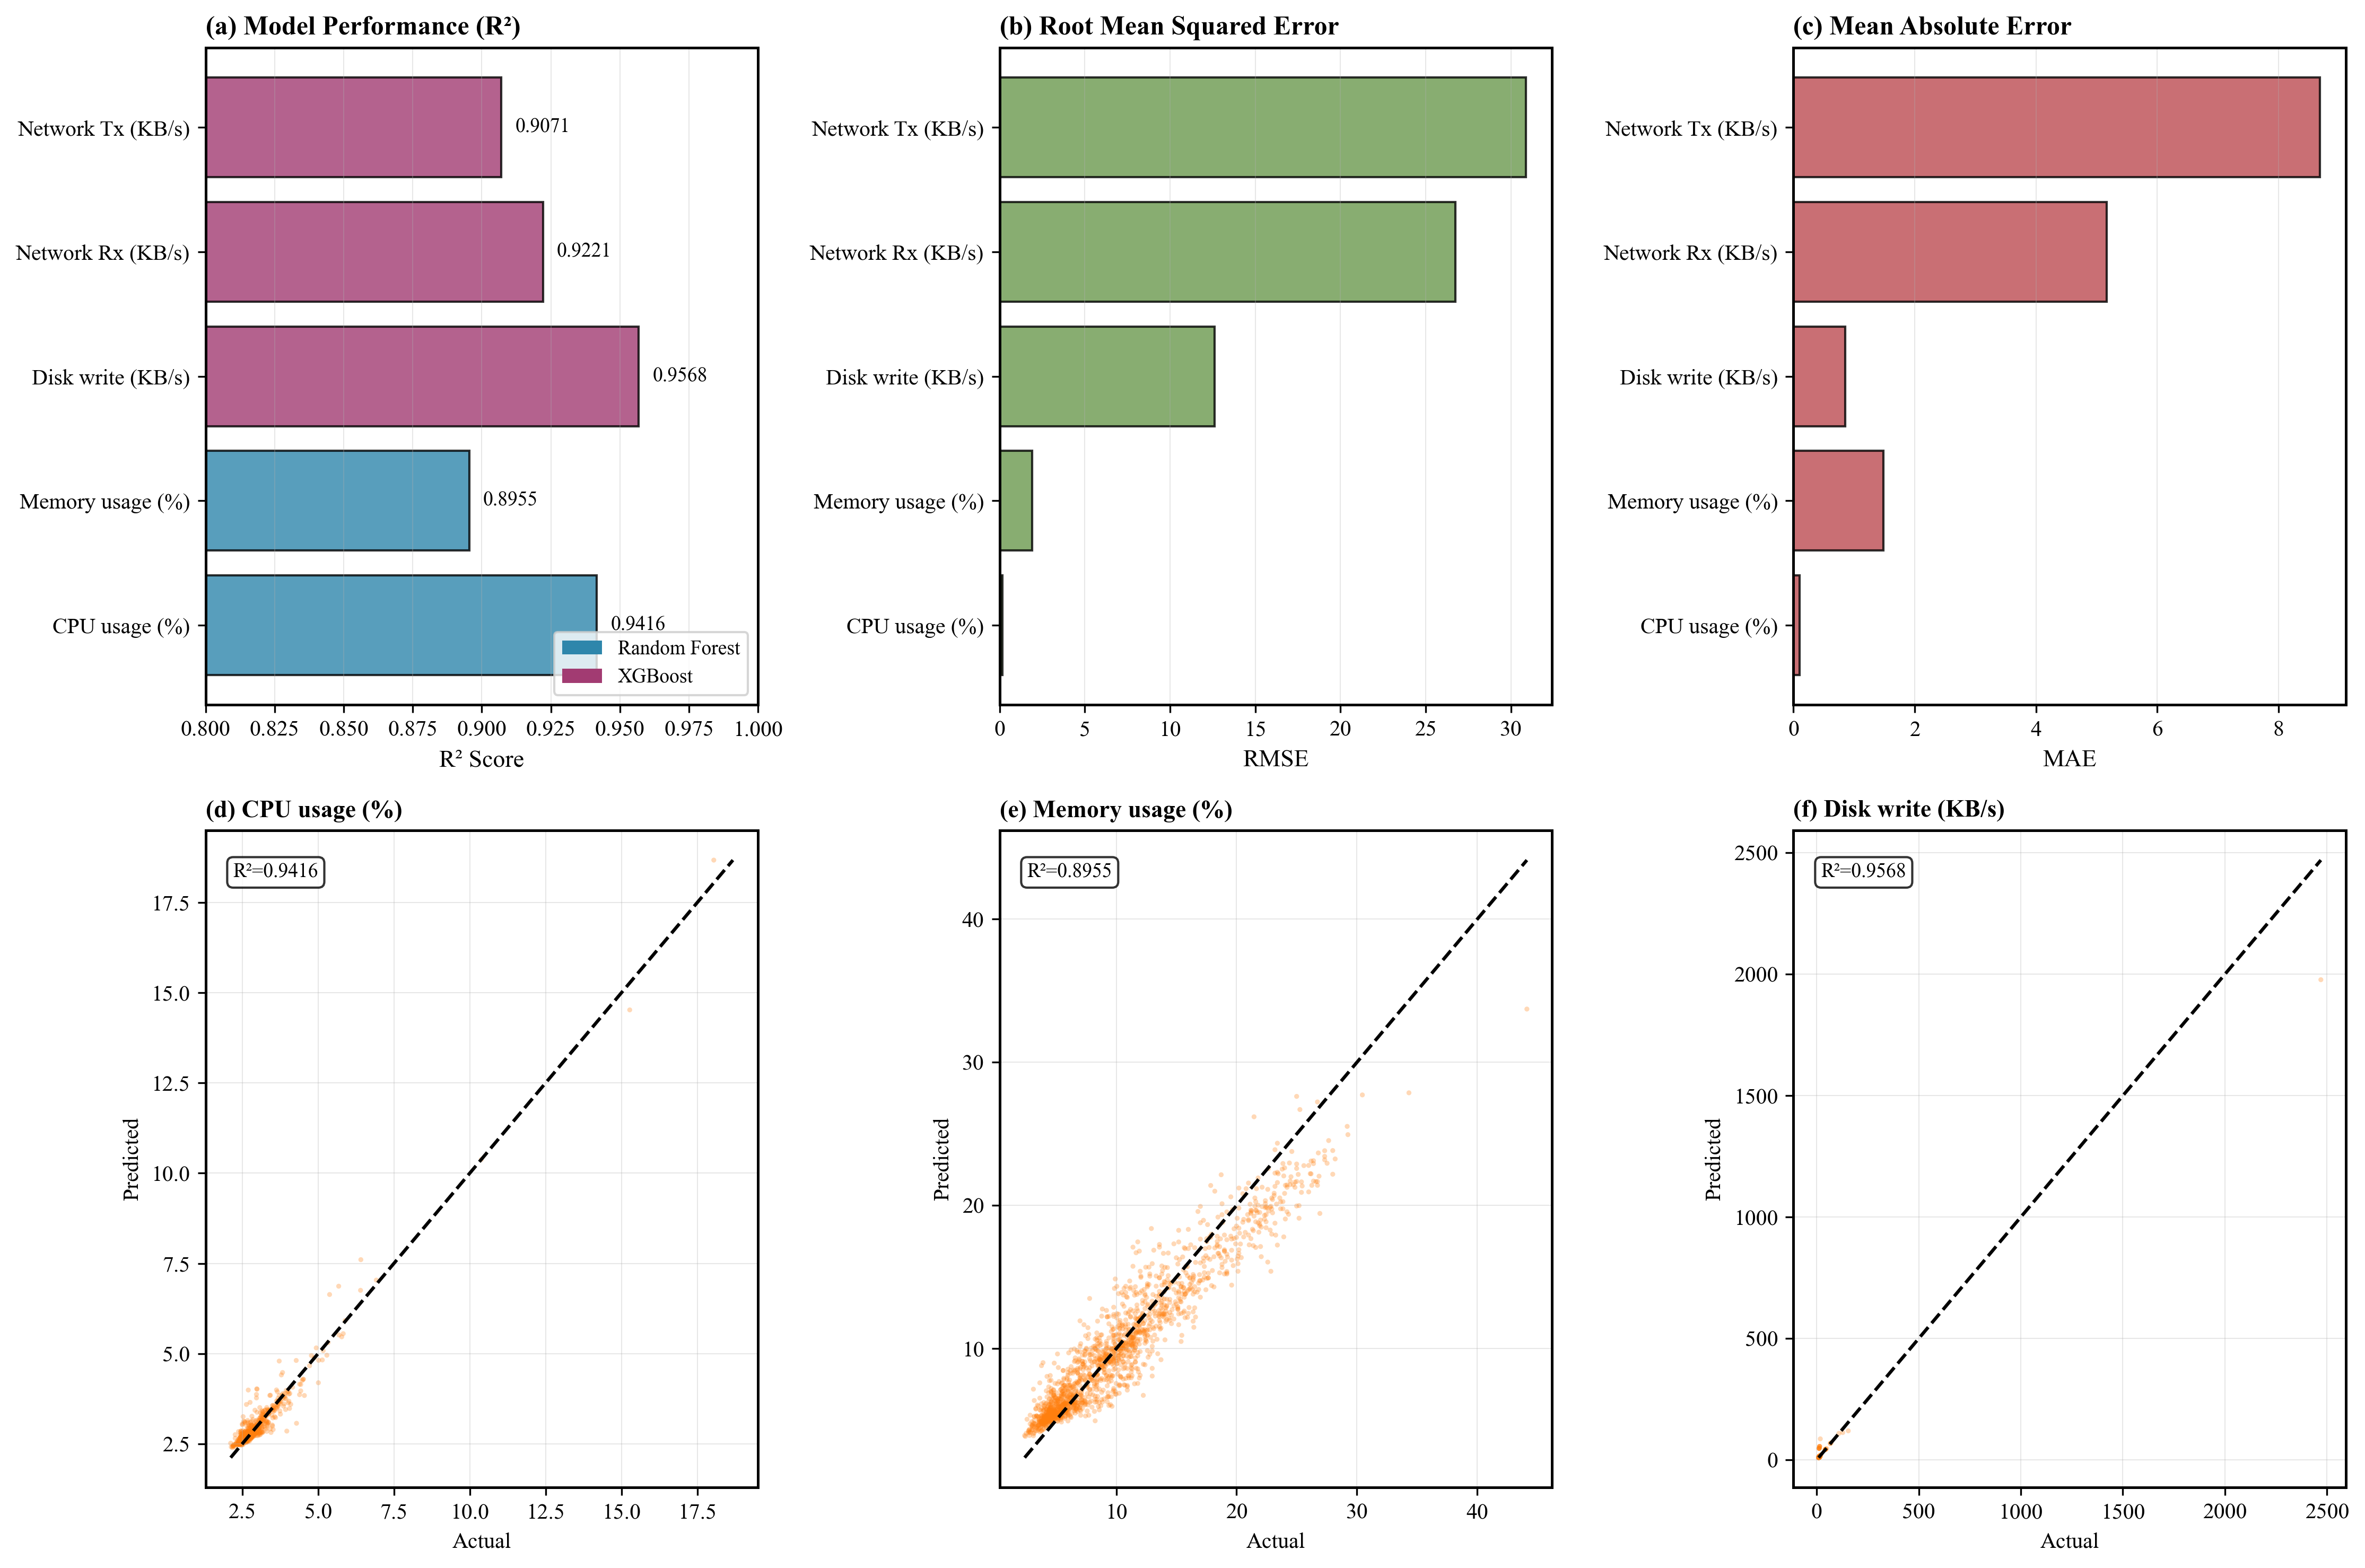
\includegraphics[width=\columnwidth]{summary_figure.png}
\captionof{figure}{Summary of model performance across all metrics, including $R^2$, RMSE, MAE, and representative scatter plots.}
\label{fig:summary_results}
\end{minipage}
\end{center}

\section{Future Work}
\label{sec:future}

Building upon the strong performance of the hybrid tree-based prediction framework, several avenues remain open for advancing predictive profiling and its integration into CECC orchestration workflows. A first direction concerns the incorporation of richer contextual and exogenous signals. Although engineered temporal features capture much of the short-term structure within CPU, memory, disk, and network behavior, CECC workloads are influenced by higher-level dynamics such as application semantics, workload phase shifts, diurnal usage cycles, maintenance windows, and user-driven activity patterns. Integrating these external signals---through log-derived event markers, service-level traces, domain-specific workload descriptors, or multi-day temporal embeddings---may further improve the accuracy and robustness of predictions, particularly for highly bursty metrics where endogenous historical patterns alone are insufficient.

A related direction involves extending the current univariate, one-step-ahead formulation to multivariate and horizon-aware forecasting. Predicting multiple resource metrics jointly may exploit cross-metric dependencies that are only partially captured through engineered features. For example, disk write bursts often precede memory pressure events, and network spikes may correlate with transient CPU peaks. Similarly, forecasting several steps into the future is valuable for anticipatory CECC operations such as early scaling, load redirection, and service migration. Multi-horizon forecasting could provide orchestration systems with more actionable lead time, enabling them to make proactive decisions rather than reacting to emerging bottlenecks.

Another promising line of investigation lies in adaptive, online, and continual learning. CECC workloads are inherently non-stationary: applications evolve, microservice deployments change over time, and resource behavior shifts due to updates, configuration adjustments, and seasonal patterns. Static models trained offline may lose accuracy as these dynamics evolve. Incremental learning techniques, concept-drift detection, and lightweight online ensemble updates could enable prediction models to remain accurate over long-running deployments. Such mechanisms align naturally with emerging dynamic profiling frameworks (e.g., DynAPM), where predictive models are continuously refined based on recent telemetry.

In parallel, there is growing interest in decentralized and privacy-preserving learning for cloud--edge ecosystems. Many CECC environments cannot aggregate raw telemetry centrally due to bandwidth constraints, privacy requirements, or local data governance policies. Future work could investigate federated training of tree-based models, hybrid split-learning approaches, or hierarchical forecast fusion between cloud and edge nodes. These techniques could maintain prediction quality while reducing communication overhead and preserving data locality.

Finally, a crucial direction involves tighter integration of predictive signals into CECC lifecycle management and orchestration systems. While the present study demonstrates the feasibility of accurate per-VM, multi-metric forecasting, the next step is to embed these predictions into dynamic Application Profile Models (APMs) and evaluate their operational impact. This includes assessing improvements in SLA compliance, quantifying reductions in scaling and migration latency, understanding trade-offs between prediction accuracy and orchestration responsiveness, and validating the end-to-end pipeline on real CECC platforms. Such closed-loop evaluations will be essential for demonstrating how prediction-driven APMs can materially enhance the reliability, efficiency, and adaptability of cloud--edge application deployments.

\section{Conclusion}
\label{sec:conclusion}

This work introduced a real-time, per-VM application performance prediction framework tailored to the heterogeneous and dynamic nature of Cloud--Edge Computing Continuum (CECC) environments. Using the large-scale, production-grade GWA-T-13 Materna traces, we demonstrated that short-term forecasting of CPU usage, memory usage, disk write throughput, and network throughput can be achieved with high accuracy when models are carefully aligned with the statistical properties of each metric. The hybrid tree-based approach developed in this study---combining Random Forest for CPU and memory with XGBoost for disk and network throughput---proved effective in capturing the diverse temporal and distributional characteristics of CECC workloads.

The results highlight several key insights for predictive CECC resource management. CPU and memory exhibit relatively smooth and periodic behavior, allowing ensemble tree models to achieve near-linear error profiles and strong generalization. Disk and network metrics, which are dominated by heavy-tailed distributions and burst-driven dynamics, benefit from the sequential error-correction and regularization mechanisms of boosted trees. Together, these models offer a practical and robust solution for multi-metric forecasting, outperforming deep recurrent architectures in this context while maintaining interpretability and computational efficiency.

Beyond predictive accuracy, the per-VM formulation aligns naturally with the operational granularity of modern microservice-based applications. The forecasts generated by the hybrid model can support proactive orchestration actions, including anticipatory autoscaling, latency-aware placement, and SLA-sensitive resource adjustments. By exposing these predictions through dynamic Application Profile Models (APMs), the approach provides a foundation for integrating predictive intelligence into CECC lifecycle management pipelines.

The study demonstrates that combining feature-rich temporal representations with model families selected for metric-specific behavior yields a scalable and effective strategy for CECC performance forecasting. Future work will deepen this integration by exploring multivariate and multi-horizon forecasting, online and continual learning, decentralized training approaches, and full closed-loop validation within real CECC orchestration systems. Such advances will enable next-generation CECC platforms to evolve from reactive monitoring toward predictive, adaptive, and autonomous management.

\section*{Funding}

This work was partially supported by the European Union’s Horizon Europe Research and Innovation programme under the AC3 project (Grant Agreement No. 101093129).

\section*{Acknowledgements}

The authors would like to thank the University of Vaasa for providing an excellent research environment and academic support throughout the development of this work. The authors also acknowledge Fingletek Oy for its technical contributions, infrastructure support, and collaboration within the AC3 project framework. The views and opinions expressed in this paper are those of the authors and do not necessarily reflect the official position of the European Union or the affiliated institutions.

\section*{Declaration of Generative AI Use}

During the preparation of this manuscript, generative artificial intelligence (AI) tools were used to assist with drafting selected sections of the text, generating portions of the code used in the study, and performing language editing and proofreading. The authors reviewed, edited, and validated all AI-assisted outputs and take full responsibility for the content, accuracy, integrity, and originality of the manuscript. No figures, images, or visual elements were generated using AI tools.

\section*{Data Availability}

The data used in this study are publicly available from the Grid Workloads Archive (GWA). Specifically, we use the GWA-T-13 Materna dataset, available at: https://atlarge-research.com/gwa-t-13/. All preprocessing scripts and model configurations used in this study are available from the corresponding author upon reasonable request.

\section*{Declaration of Competing Interest}

The authors declare that they have no known competing financial interests or personal relationships that could have appeared to influence the work reported in this paper.

\printcredits

\begin{thebibliography}{00}

\bibitem{b1}
S. Islam, J. Keung, K. Lee, and A. Liu,
Empirical prediction models for adaptive resource provisioning in the cloud,
Future Generation Computer Systems (2020).

\bibitem{b2}
P. Sharma, D. Irwin, and P. Shenoy,
Predicting Network Throughput for Cloud Applications,
in: Proc. IEEE INFOCOM, 2021.

\bibitem{b3}
A. Ahmad, S. Choi, and Y. Kim,
Time-series prediction of cloud workloads using ARIMA,
IEEE Access (2020).

\bibitem{b4}
Z. Huang, C. Fang, and L. Meng,
Memory Usage Forecasting in Virtualized Clouds Using Seasonal ARIMA,
Journal of Systems Architecture (2021).

\bibitem{b5}
J. Chen, R. Duan, and B. Li,
Multivariate workload prediction in cloud data centers using VAR models,
IEEE Transactions on Services Computing (2022).

\bibitem{b6}
V. Pandey and R. Tiwari,
Forecasting Web Traffic Using Holt--Winters Model,
Applied Soft Computing (2020).

\bibitem{b7}
W. Zhang, Y. Chen, and M. C. Gursoy,
Machine learning-based resource usage prediction for cloud VMs,
IEEE Transactions on Cloud Computing (2021).

\bibitem{b8}
X. Zhao, L. Peng, and H. Wang,
Disk I/O performance prediction using XGBoost in cloud environments,
Future Generation Computer Systems (2022).

\bibitem{b9}
L. Su, Y. Ji, and J. Zeng,
Network Traffic Forecasting in Backbone Networks Using LightGBM,
Computer Networks (2023).

\bibitem{b10}
S. Kim and J. Lee,
Support Vector Regression for predicting cloud VM resource usage,
in: Proc. IEEE ICPADS, 2020.

\bibitem{b11}
R. Ghosh and A. Chattopadhyay,
LSTM-based cloud workload prediction,
IEEE Transactions on Cloud Computing (2021).

\bibitem{b12}
M. Bharathi and R. Buyya,
Deep Learning Models for Microservices Resource Forecasting in Kubernetes,
Journal of Parallel and Distributed Computing (2022).

\bibitem{b13}
H. Wang and F. Xu,
GRU-based latency prediction for mobile edge computing,
IEEE Internet of Things Journal (2021).

\bibitem{b14}
H. Xu and J. Liu,
CNN--LSTM Hybrid Models for Network Traffic Prediction,
IEEE Transactions on Network Science and Engineering (2022).

\bibitem{b15}
S. Li et al.,
Informer: Beyond Efficient Transformer for Long Sequence Time-Series Forecasting,
in: Proc. AAAI, 2021.

\bibitem{b16}
J. Sun and Y. Chen,
Autoformer for Cloud Workload Forecasting,
in: Proc. IEEE ICDCS, 2023.

\bibitem{b17}
Q. Yang and X. Guo,
Federated LSTM for Distributed Edge Workload Prediction,
IEEE Transactions on Mobile Computing (2024).

\bibitem{b18}
Y. Li and K. Wang,
On-device GRU inference for resource prediction in edge computing,
IEEE Transactions on Computers (2023).

\bibitem{b19}
J. Zeng and A. Li,
Cloud--Edge Collaborative Learning for Latency Prediction in Video Analytics,
in: Proc. ACM/IEEE Symposium on Edge Computing (SEC), 2022.

\bibitem{b20}
S. Mohsen, A. Elkaseer, and S. Scholz,
Industry 4.0-Oriented Deep Learning Models for Human Activity Recognition,
IEEE Access (2021).

\end{thebibliography}

\end{document}